\documentclass[12pm,twosides,onecolumn,openany]{book}
\usepackage{graphicx} 
\usepackage[catalan]{babel}
\usepackage{emptypage}
\usepackage{hyperref}
\usepackage{mathtools}
\usepackage{blindtext}
\usepackage[utf8]{inputenc}
\usepackage{caption}
\usepackage{subcaption}
\usepackage{wrapfig}
\usepackage[a4paper]{geometry}
\geometry{top=2.5cm, bottom=2.5cm, left=2.5cm, right=2.5cm}
\usepackage{fancyhdr}
\pagestyle{fancy}
\usepackage{amsmath}
\usepackage{amssymb}
\usepackage{amsfonts}
\providecommand{\norm}[1]{\lVert#1\rVert}
\hypersetup{colorlinks=true,urlcolor=blue,linkcolor=blue}
\usepackage{multirow}
\usepackage{multicol}
\usepackage{rotating}
\usepackage{titlesec}
\usepackage{tcolorbox}
\tcbuselibrary{breakable}
\usepackage{listings}
\usepackage{xcolor}

% Configuració del títol d'exemple:
\title{Titol d'exemple}
\author{Onofre A.}
\date{Febrer 2025}
% Color de fons dels listings
\definecolor{bgcolor}{rgb}{0.94,0.94,0.94}

% Colors per a interpretar LaTeX al PDF
\definecolor{codegray}{rgb}{0.5,0.5,0.5}
\definecolor{codeblue}{rgb}{0,0,1}
\definecolor{codegreen}{rgb}{0,0.6,0}
\definecolor{codered}{rgb}{0.8,0,0}

% Configuració per a que listings entengui LaTeX
\lstdefinelanguage{LaTeX}{
    keywords={documentclass, usepackage, begin, end, chapter, section, subsection, textbf, textit, title, author, date, maketitle, tableofcontents, includegraphics, caption, label, ref, cite, pagestyle, thispagestyle, newpage, texttt, textsc, textsf},
    keywordstyle=\color{codeblue}\bfseries,
    morekeywords=[2]{include, input, newcommand, renewcommand, geometry, textcolor, footnote, emph},
    keywordstyle=[2]\color{codered}\bfseries,
    sensitive=true,
    comment=[l]{\%},
    morecomment=[s]{/*}{*/},
    commentstyle=\color{codegray}\itshape,
    string=[b]",
    stringstyle=\color{codegreen}
}

% Configuración global de la font per a listings
\lstset{
    language=LaTeX,
    basicstyle=\ttfamily\small,
    keywordstyle=\color{codeblue}\bfseries,
    backgroundcolor=\color{bgcolor},
    commentstyle=\color{codegray}\itshape,
    stringstyle=\color{codegreen},
    breaklines=true,
    breakindent=0pt,
    framexrightmargin=0.05\textwidth,
    linewidth=0.95\textwidth,
    frame=none,
    captionpos=b,
    numbers=left,
    numbersep=5pt,
    numberstyle=\tiny\color{gray},
    showspaces=false,
    showstringspaces=false,
    tabsize=4,
    inputencoding=utf8
}

\newenvironment{Figura}
  {\par\medskip\noindent\minipage{\linewidth}}
  {\endminipage\par\medskip}

\titleformat{\section}  % comando de sección a formatear
  {\fontsize{14}{16}\bfseries} % formato para toda la línea
  {\thesection} % cómo mostrar el número
  {0.4em} % espacio entre el número y el texto
  {} 
  [] 

% Comptador d'exemples
\newcounter{exemple}[chapter] 
\renewcommand{\theexemple}{\thechapter.\arabic{exemple}}
\newcommand{\exemple}[1]{
    \refstepcounter{exemple}
    \textbf{Exemple \theexemple} #1
}

% Configuració de la capçalera
\fancyhf{}
\fancyhead[RO,LE]{\rightmark}
\fancyhead[LO,RE]{\leftmark}
\fancyfoot[RO,LE]{\thepage}
\fancyfoot[LO,RE]{Curs d'Introducció a LaTeX}

\renewcommand{\chaptermark}[1]{\markboth{\thechapter.\ #1}{}}
\renewcommand{\sectionmark}[1]{\markright{\thesection.\ #1}}

\graphicspath{ {images/} }

\begin{document}
\newpage
\thispagestyle{empty}
\begin{titlepage}
    \centering
    \vspace*{\fill}  
    {\Huge \textsc{Curs d'Introducció a \LaTeX{}} \par}
    \vspace{1cm}
    {\Large Optica't UAB \par}
    \vspace{0.5cm}
    {\large Versió 1.0 \par}
    \vspace{5cm}
    \vspace*{\fill} 
\end{titlepage}


\newpage

\thispagestyle{empty}
Benvolguts i benvolgudes a aquest text introductori de LaTeX. Som Optica't, un grup de divulgació d'òptica física format per estudiants de la Universitat Autònoma de Barcelona. Aquest text està pensat per a facilitar l'aprenentatge d'aquesta eina a alumnes que comencin els seus estudis universitaris. Clarament, està orientat a graus científics, el nostre aprenentatge de LaTeX es basa en les necessitats i la curiositat que hem desenvolupat al llarg dels cursos en carreres com física o nanociències. Tot i això, pensem que LaTeX és una eina molt útil per a més disciplines i esperem que molta gent pugui fer profit d'aquest curs.

\newpage
\tableofcontents
\pagestyle{empty}
\newpage
Agraïments
\newpage
\pagestyle{fancy}
\chapter{Introducció i conceptes bàsics}
\thispagestyle{empty}

Dediquem aquest capítol a explicar des de zero com funciona LaTeX i com podem començar a crear els nostres primers documents. La finalitat del capítol és que us quedeu amb els conceptes bàsics de com funciona l'eina, la seva sintaxi, els possibles errors que trobareu, etc.

\section{Què és LaTeX i la seva utilitat}
LaTeX és un editor de textos que funciona de forma similar a un llenguatge de programació compilat. Està basat en el llenguatge de baix nivell \TeX{}, i està pensat principalment per a escriure textos científics de forma senzilla i elegant. La filosofia d'aquesta eina és que qui redacti no es preocupi del format del document, només en què ha d'escriure. A diferència d'un editor de textos \textsc{WYSIWYG} (en anglès, 'el que veus és el que obtens') al treballar amb LaTeX no podem veure el resultat del que redactem al moment d'escriure-ho. En LaTeX es treballa directament amb codi i després un compilador ho interpreta i genera un resultat (per exemple imprimeix el document per pantalla o genera un arxiu \texttt{.pdf}).\\\\
En un principi pot semblar que escriure en codi i no veure què és el que estem generant és contraproduent i pot fer menys atractiva la idea de treballar amb aquest editor i no amb altres més populars. Però, com veureu al llarg d'aquest text, aquest desavantatge queda opacat per la quantitat d'eines útils i de personalització que s'obtenen en treballar amb LaTeX.\\\\
Aquest curs se centra a abastar tot el necessari per a començar a escriure textos científics, com ara lliuraments de diverses assignatures de la carrera o per al treball de fi de grau. Però, en ser només un text introductori, no podrem explicar totes les eines que ofereix LaTeX bàsic i encara menys totes les eines que ha creat la comunitat. És necessari dir també que la utilitat d'aquest editor de textos va més enllà dels textos científics semblants a \textit{papers}. LaTeX té incorporades eines per a escriure llibres, per a escriure música, per a fer presentacions... Us convidem a informar-vos més enllà d'aquest text perquè podeu jugar amb totes les possibilitats que ofereix LaTeX tot i que no estudieu a cap branca científica.
\section{Entorns per a treballar amb LaTeX}
Per començar a treballar amb LaTeX primer necessitem saber on! És a dir, necessitem saber quin és el nostre entorn de treball. Igual que passa amb els llenguatges de programació, podem córrer LaTeX a dins d'una gran varietat d'entorns. Cada entorn és lleugerament diferent de l'altre, les seves característiques depenen de la versió i de quin sigui el flux de treball pensat específicament per a aquell entorn. Escollir un bon entorn pot arribar a ser una mica enrevessat, per tant, per a facilitar la tasca a les persones que encara no han fet servir LaTeX o que no estiguin familiaritzades en treballar amb programes de manera local centrarem el curs en l'entorn d'Overleaf. Sense ser exhaustius també parlarem sobre altres entorns com algunes eines d'escriptori o a escriure directament en un document de text amb eines més específiques de programació.\\\\
Per al lector o lectora que ja tingui experiència amb Overleaf i vulgui fer servir les altres eines, pròximament crearem una guia que complementi aquest curs amb més informació, de moment ens centrarem en que pugueu escriure el vostre primer document en LaTeX.
\subsection{Overleaf}
L'entorn per exce\lgem ència per a aprendre LaTeX i per a fer petits projectes co\lgem aboratius és Overleaf. Per a fer-ho servir no cal insta\lgem ar-se res, només necessites connexió a internet i un usuari. Overleaf és un entorn de LaTeX en línia pensat per a fer més fàcil la co\lgem aboració entre usuaris a l'hora de crear un document compartit. Els seus avantatges són:
\begin{itemize}
    \item No requereix cap insta\lgem ació, només tenir un compte. Per a poder accedir a un compte d'Overleaf només necessiteu un correu electrònic i entrar a la web oficial\footnote{Us deixem l'enllaç vigent actualment: \url{https://es.overleaf.com}}

    \item Interpreta el codi fins i tot si aquest conté algun petit error

    \item Permet treballar conjuntament amb diverses persones\footnote{Actualment (inici del 2025) la limitació per a editar el mateix projecte d'Overleaf es limita a dos usuaris. La resta d'usuaris que entrin al projecte només poden llegir-ho.}

    \item Permet classificar els teus projectes amb etiquetes

    \item Té insta\lgem ats alguns paquets que el LaTeX pur no té per defecte

    \item Té un sistema de navegació i una visualització del log de compilació intuïtius 

    \item Té integrades algunes eines que faciliten la generació de codi, com ara botons o \textit{short cuts} que canvien el format del text com en Word o un generador de taules buides

    \item Proporciona un editor visual on es pot treballar en un entorn semblant a un editor WYSIWYG
\end{itemize}
Com aquesta serà l'eina que farem servir a la resta del curs, explicarem una mica més sobre com funciona. Un cop tinguem obert un compte podrem crear un nou projecte des del menú principal. Overleaf ofereix moltes plantilles preestablertes, però per a aprendre treballarem amb una plantilla buida. Un cop obert el nou projecte en blanc veurem la següent pantalla:

\begin{figure}[h]
    \centering
    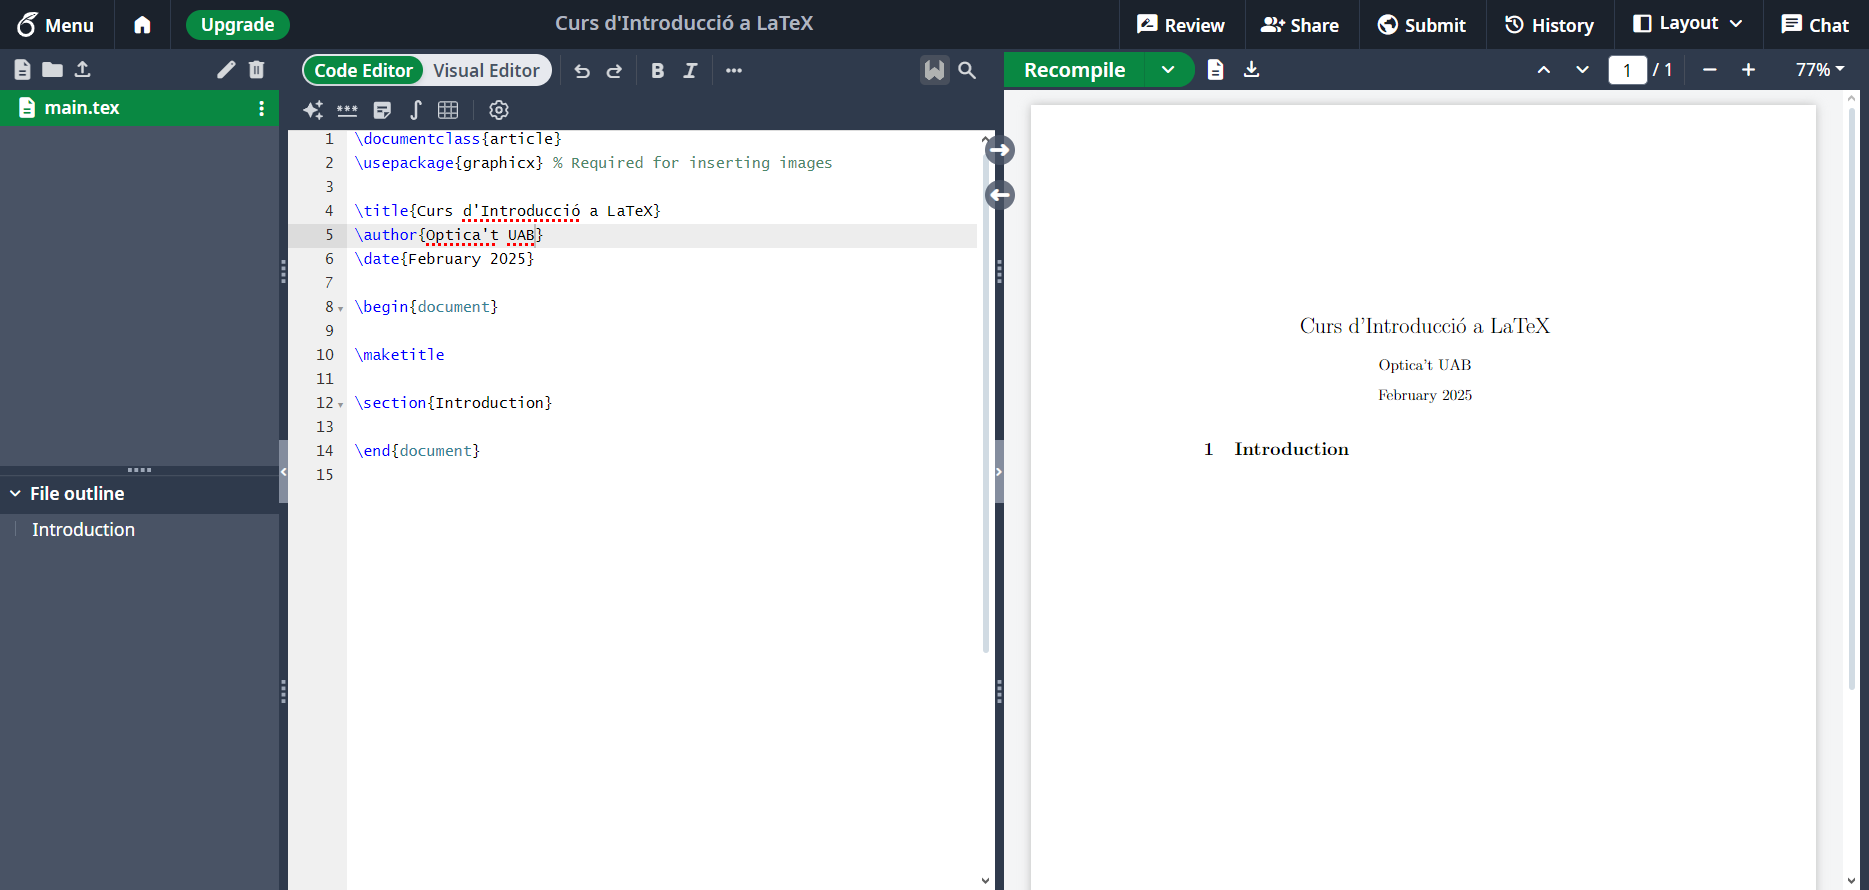
\includegraphics[width=0.95\linewidth]{../Text principal/Imatges/captura_nou_projecte.png}
    \caption{Entorn de treball d'Overleaf per a un projecte en blanc.}\label{fig:entorn_Ovlf_blanc}
\end{figure}

\noindent Observem de la Figura \ref{fig:entorn_Ovlf_blanc} que l'entorn se separa en tres parts. A l'esquerra del tot observem un menú, l'explorador d'arxius i de projecte. Aquest explorador funciona com a un gestor de carpetes i d'arxius, molt similar a l'explorador d'arxius de Windows. A la part superior de l'explorador aniran apareixent els arxius que fem servir al projecte. Podem mantenir un ordre d'aquests arxius utilitzant carpetes i canviant el nom de cada arxiu com vulguem. A la part inferior de l'explorador apareixerà un llistat de títols que ens serveixen per a moure'ns pel projecte de forma més senzilla, expliquem el seu funcionament amb més detall a la secció \ref{sec:cap_sec_subsec}.\\\\
A la dreta de la pantalla s'observa un visor pdf. Aquest visor permet veure per pantalla com va quedant el document que estem generant amb el codi que hem escrit. Notareu que a la part superior esquerra del visor hi ha un botó verd on posa \texttt{Recompile}. Cada cop que vulguem actualitzar el pdf amb la informació que hem escrit en codi hem de fer click a \texttt{Recompile}\footnote{No cal fer click sempre, existeixen dues alternatives. La primera és fer servir \textit{short cuts}, és a dir, prémer \texttt{Ctrl + s} o bé \texttt{Ctrl + Enter}. La segona és activar la funció automàtica de recompilat. Podeu accedir a aquesta opció desde el botó \texttt{Recompile}, prement la fletxa que té al costat.}. Diem a aquesta acció recompilar o compilar el codi.\\\\
Entre l'explorador i el visor tenim l'editor de text. Aquest editor és igual que qualsevol altre en programació. Allà és on escrivim totes les línies de codi necessàries per a generar el nostre document. Tot i això, aquesta finestra intermitja no sempre farà d'editor. Overleaf permet treballar amb més tipus d'arxiu que els de LateX com per exemple imatges. Per tant és més encertat pensar en l'editor com un entorn dinàmic de treball i no només com un simple editor de text.\\\\
Es pot configurar la visibilitat tant de l'editor com del visor pdf a partir de les opciones del desplegable \texttt{Layout}. Aquestes opcions deixen només visible un dels dos, els dos o permet separar-los en finestres diferents del navegador (això és útil si per exemple treballem a doble pantalla).
\subsection{LaTeX d'escriptori}
A part de l'Overleaf, també existeix la versió per escriptori de LaTeX sense necessitat de connexió a la xarxa.El procés de baixada i insta\l.lació pot resultar una mica enrevessat i feixuc si és el primer cop que es treballa amb programes com aquest.\\\\
El LaTeX d'escriptori funciona lleugerament diferent que els programes d'edició de textos que estem acostumats. Per fer-lo funcionar necessitem: el \textbf{MiKTeX} i el \textbf{TexMaker}. 
El primer funcionarà com a administrador de paquets els quals haurem d'insta\l.lar en el nostre ordinador per fer-ne ús. El segon és l'editor en sí, on hi escriurem els nostres documents.\\\\
Per baixar-se el MiKTeX és el següent enllaç on hi ha l'opció per a Windows, Linux i Mac \url{https://miktex.org/download} i per baixar-se el TexMaker \url{https://www.xm1math.net/texmaker/}. Per facilitar la insta\l.lació, crearem una carpeta en el nostre ordinador i en allà serà on hi posarem el MiKTeX.
\begin{itemize}
    \item Quan comencem a insta\l.lar se'ns obrirà una pestanya que ens demanarà \textit{Prefered Paper} en el qual hi posarem la opció A4 i a \textit{Install missing packages} triarem l'opció \textit{Ask me first}. Això vol dir que cada vegada que el MiKTeX detecti que estem utilitzant un paquet que no el tenim insta\l·lat, ens demanarà permís per insta\l.lar-lo. Cal remarcar que el procés d'insta\l.lació trigarà el seu temps així que millor prendre-s'ho amb calma.
    \item Quan aparegui l'\textit{Update Check}, deseleccionem l'opció de \textit{Check for updates now} així agilitzarem el procés. 
\end{itemize}
D'aquesta manera, ja tenidrem el MiKTeX insta\l.lat. Ara falta el TexMaker que ja té una insta\l.lació més normal.\\\\
Un cop tinguem el MiKTeX i el TexMaker en el nostre ordinador podrem començar a escriure el nostre primer document en el LateX d'escriptori. El funcionament del programa
és molt semblant a l'Overleaf amb la única diferència que s'ha d'anar guardant. Això sí, serà necessari que el nostre ordinador disposi d'un lector de PDF i un administrador de referències com ara el JabRef \url{https://www.jabref.org/}.\\\\
És recomanable, que cada document es crei en una carpeta diferent ja que quan guardem els nostres documents, es guarda la versió PDF, versió de TextMaker i llavors altres arxius que no ens interessen (quan treballem a un nivell introductori, es clar). Cada vegada que compilem el document, l'arxiu PDF es reescriurà amb la nova informació.
\subsection{Eines alternatives}
Per a la gent més experimentada o amb més interés en la programació deixem el següent entorn que, tot i potser semblar més complicat de fer servir, permet personalitzar completament el teu entorn de treball. LaTeX és un llenguatge, no un programa, per tant desde qualsevol editor de text podem escriure en LaTeX i, fent servir el compilador corresponent podrem generar la sortida que vulguem. Ara bé, existeixen eines que faciliten aquesta feina i ens permeten configurar el nostre entorn de forma més visual. Podriem fer una llista enorme amb eines de visualització útils i personalitzables, però una de les més populars (i des de la que s'està redactant aquest text) és Visual Studio Code. La instalació i configuració d'aquest entorn queda fora dels proposits d'aquest curs, però us convidem a informar-vos una mica sobre aquesta eina ja que no serveix només per a LaTeX. Visual Studio Code permet treballar amb LaTeX (i molts més llenguatges) en local, té integrat un explorador de directoris molt visual (no cal barallar-se amb la bash per a navegar per les carpetes) i permet afegir extensions pensades per a treballar amb LaTeX.
\section{Estructura bàsica d'un document}
De forma similar a un llenguatge de programació quan escrivim un document en LaTeX necessitem seguir un cert ordre i respetar una sintaxi concreta per a que el compilador pugui comprendre i traduïr correctament el nostre document. Aquestes normes que s'han de seguir no són complicades, de fet amb Overleaf són similars a escriure en Word. Com hem comentat abans, LaTeX està pensat per a que no ens haguem de preocupar per la forma sinó més per qué escrivim, per tant és aquí on hi ha la diferència principal amb altres eines d'edició de textos. 
\subsection{Sintaxi}
L'estructura d'un document de LaTeX se separa en dues parts ben diferenciades:
\begin{itemize}
    \item \textbf{Preàmbul}: a on escrivim la ``configuració'' del document
    \item \textbf{Text principal}: a on escrivim el cos del document
\end{itemize}
Separem aquestes dues parts de forma explícita, reservant sempre les primeres línies de codi per al preàmbul i la resta per al text principal. Veiem com a exemple el codi que escriu Overleaf per defecte quan obrim un document en blanc:\\\\
\exemple{\label{ex:\theexemple}}\footnote{Tant Overleaf com LaTeX permet fer servir accents escrits directament amb el teclat o amb codi (ho veurem més endavant). Però, l'entorn que fem servir per a escriure els exemples no els detecta correctament. Això no serà un problema per a volsaltres a l'hora de redactar un document sense aquest recurs. Si us plau, feu servir accents.}
\begin{lstlisting}
    \documentclass{article}
    \usepackage{graphicx} % Required for inserting images

    \title{Curs d'Introduccio a LaTeX}
    \author{Optica't UAB}
    \date{February 2025}

    \begin{document}

    \maketitle

    \section{Introduction}

    \end{document}
\end{lstlisting}
Des de la primera línia fins a la setena és el preàmbul. La resta és el text principal i comença amb el comandament \texttt{\textbackslash begin\{document\}}. 
L'exemple \ref{ex:1.1} ens permet veure els tres tipus de comandaments bàsics del preàmbul i com s'estructura un document. El preàmbul de l'exemple comença declarant a la primera línia el tipus de document que estem redactant. Seguidament, a la segona, declara el paquet \texttt{graphicx}. Els últims tres comandaments configuren tres objectes predefinits (el títol, l'autor i la data). Veiem doncs que al preàmbul els comandaments bàsics que podem fer servir són:
\begin{itemize}
    \item[-] Declaració de tipus de document
    \item[-] Declaració de paquets
    \item[-] Configuració d'entorns pre-establerts
\end{itemize}
Parlarem amb més detall d'aquests comandaments a les següents seccions (\ref{sec:tipus_de_document}, \ref{sec:paquets} i \ref{sec:entorns}). La resta del document, alló que es plasmarà al compilar, es redacta en un entorn delimitat pels comandaments \texttt{\textbackslash begin\{document\}} i \texttt{\textbackslash end\{document\}}. El codi que hi ha escrit entre aquests delimitadors serveix per a imprimir al document el títol i el títol de la secció anomenada ``Introduction''. Més endavant ens interessarem per aquests comandaments. Encara més important per a aquesta part del codi és com es redacta text pla per a que s'imprimeixi com volem per pantalla. Veiem-ne alguns exemples:\\\\
\exemple{\label{ex:\theexemple}}
\begin{lstlisting}
    \documentclass{article}

    \begin{document}
        Aixo s'escriu en text pla, amb una mida de font standar i amb 
        uns marges per defecte.
    \end{document}
\end{lstlisting}
\textbf{Sortida:}
\begin{tcolorbox}[colframe=black, colback=white, sharp corners, width=\textwidth,boxrule=0.2mm]
    Aixo s'escriu en text pla, amb una mida de font standar i amb uns marges per defecte.
\end{tcolorbox}
Com veiem el text s'escriu justificat a l'amplada del document i amb una mida de text normal. La mida i el tippus de lletra es pot modificar tant a la configuració del preàmbul com al mateix codi (veure secció \ref{sec:format_del_text_pla}). Si tenim més text aquest s'adaptarà en forma de paràgraf. Existeixen diverses formes de separar dos paràgrafs i cada forma crea un salt de línia de diferent mida i genera o no indentació per defecte.\\\\
\exemple{\label{ex:\theexemple}}
\begin{lstlisting}
    \documentclass{article}

    \begin{document}
        Aquest es un text d'exemple que omplira l'amplada del document formant un unic paragraf. Podem separar-ho en altres paragrafs de diferents maneres.\\
        Aquest paragraf esta separat per $\backslash\backslash$. S'aplica un salt de linia normal, amb una separacio igual a la d'un salt de linia del mateix paragraf i no aplica indentacio.

        Deixar una linia en blanc tambe genera un altre paragraf com al escriure $\backslash\backslash$ pero a mes aplica indentacio. Si LaTeX detecta que hi ha mes d'un espai en blanc normalment avisa amb un error de sintaxi. Overleaf permet fer aquest espais en blanc i ho interpreta com a un de sol.Podem generar el mateix efecte separant el paragraf amb el comandament $\backslash$par. LaTeX quan es troba aquest comandament enten que s'ha acabat un paragraf i que lo que ve a continuacio pertany a un seguent paragraf. \par Per exemple aquest text esta separat pel comantament $\backslash$par.\\\\
        Aquest darrer paragraf se separa amb quatre $\backslash$. Aquesta forma de separar paragrafs no genera indentacio i crea un salt de linia mes gran, fent que el text se separi en dos de forma mes visual. 
    \end{document}
\end{lstlisting}
\textbf{Sortida:}
\begin{tcolorbox}[colframe=black, colback=white, sharp corners, width=\textwidth,boxrule=0.2mm,parbox=false]
    Aquest es un text d'exemple que omplira l'amplada del document formant un unic paragraf. Podem separar-ho en altres paragrafs de diferents maneres.\\
    Aquest paragraf esta separat per $\backslash\backslash$. S'aplica un salt de linia normal, amb una separacio igual a la d'un salt de linia del mateix paragraf i no aplica indentacio.

    Deixar una linia en blanc tambe genera un altre paragraf com al escriure $\backslash\backslash$ pero a mes aplica indentacio. Si LaTeX detecta que hi ha mes d'un espai en blanc normalment avisa amb un error de sintaxi. Overleaf permet fer aquest espais en blanc i ho interpreta com a un de sol.Podem generar el mateix efecte separant el paragraf amb el comandament $\backslash$par. LaTeX quan es troba aquest comandament enten que s'ha acabat un paragraf i que lo que ve a continuacio pertany a un seguent paragraf. \par Per exemple aquest text esta separat pel comantament $\backslash$par.\\\\
    Aquest darrer paragraf se separa amb quatre $\backslash$. Aquesta forma de separar paragrafs no genera indentacio i crea un salt de linia mes gran, fent que el text se separi en dos de forma mes visual. 
\end{tcolorbox}

El detall de com escriure $\backslash$ dins del codi per a que s'imprimeixi correctament ho explicarem més endavant. A l'exemple \ref{ex:1.3} podem veure quatre formes de separar paràgrafs. L'ús d'un salt o altre ve a gust de qui està redactant el document. En aquest text, per exemple, normalment separem els paragrafs amb $\backslash\backslash\backslash\backslash$ per a obtenir un efecte visual més polit. La separació de paràgrafs de vegades ve condicionada pel que té el paràgraf al seu voltant, usualment pel codi just a sobre d'ell\footnote{Això ho veureu a mesura que escriviu documents en LaTeX, lo més usual és veure-ho quan es comença un paràgraf després de posar una figura o una taula. Per exemple, al finalitzar l'exemple \ref{ex:1.3} comença un paràgraf amb indentació automàtica.}. En cas de voler afegir o treure una indentació desitjada o no podem fer servir el comandament $\backslash$\texttt{indent} o $\backslash$\texttt{noindent}.\\\\
La indentació a LaTeX pot portar una mica de confusió no només amb el que s'imprimeix en pantalla al genrar el resultat, sinó també amb la indentació dins del propi codi. L'estructura del codi que escrivim ve imposada pel fet que hem de fer entendre al compilador què volem que surti exactament. Però, per a poder facilitar la nostra lectura del codi podem fer servir una jerarquia amb la indentació dins del codi. Fixem-nos novament en l'exemple \ref{ex:1.3}, el text que s'acabarà imprimint al document es troba indentat respecte als delimitadors del document (el \texttt{begin} i el \texttt{end}). Podriem escriure aquest codi sense aplicar aquesta indentació i el resultat per pantalla acabaria sent el mateix que abans. Aquesta indentació global el compilador la ignora, però a nosaltres ens és útil per a saber que aquella part del codi pertany al document. En cas de ternir més entorns a dins del codi (com veurem a la secció \ref{sec:entorns}) podem aprofitar aquesta indentació per a poder escriure un codi més polit que pugui ser fàcilment entés tant pel compilador com per a qui escriu o revisa el codi.
\subsubsection{Paraules reservades i comandaments}
Com heu pogut observar als exemples que hem posat fins ara hi ha algunes paraules que les hem posat en color blau. Semblant a un llenguatge de programació, LaTeX té un conjunt de paraules i simbols reservats per a que el compilador entengui si estem escrivint text pla o si estem donant una ordre concreta. Els comandaments (ja siguin del preàmbul o a dins del text o entorns matemàtics) venen declarats començant pel símbol ``$\backslash$''\footnote{És per aquest motiu que no hem escrit directament el símbol al codi per a que s'imprimeixi en la sortida del document, ja que LaTeX ho interpretaria com a un comandament i no com a un símbol}. Entorns visuals com Overleaf faciliten la tasca de saber quines són aquestes paraules reservades canviant el seu color al codi o fins i tot fent prediccions del codi que volem escriure.\\\\
No és viable aprendre de forma activa quines són aquestes paraules (no recomenem provar-ho, és una tasca molt farragosa). Lo més útil és practicar i amb el temps acostumar-se a la forma intuituva que té LaTeX de seleccionar aquestes paraules, ja que normalment són instruccions literals en anglès. Al llarg del curs explicarem algunes d'aquestes paraules reservades i a l'Annex deixarem algunes taules amb exemples útils que podeu fer servir al vostre dia a dia.\\\\
A més, veureu que acompanyant a aquestes paraules reservades normalment apareixen \{ \} o [ ]. Entre claus normalment s'escriu l'argument de la funció que estiguem cridant amb la paraula reservada. Entre claudators normalment s'escriuen les opcions de configuració de la funció.
\subsection{Tipus de document}\label{sec:tipus_de_document}
Fixem-nos ara en la primera línia del preàmbul. Com hem dit aquest comandament declara quin tipus de document estem escrivint. Segons com configurem aquesta línia, el text que redactem sortirà amb una configuració predefinida o altre. Aquesta configuració és molt bàsica, però pot portar a problemes que semblen que no tenen solució si no es té en compte qué hem configurat i que no. Existeixen molts tipus de documents que enten LaTeX, comentem per sobre els més comuns:
\begin{itemize}
    \item \textbf{\texttt{article}} - Aquest és el tipus de document que normalment fareu servir a la carrera. Està pensat per a escriure documents científics curts, de forma que permet estructurar el text en seccions.
    \item \textbf{\texttt{report}} - En cas de necessitar fer un article més llarg podeu fer servir aquest tipus de document. Un \texttt{report} permet a més de seccions separar el text en capítols.
    \item \textbf{\texttt{book}} - Aquest és el tipus de document que fem servir per a redactar aquest curs. Treballa de forma similar a un report (és un text llarg i amb capítols) pero afegeix detalls necessaris per a estructurar un llibre. Un exemple molt clar d'això és que de forma automàtica genera l'espai en blanc adient per a que els capítols començin en una pàgina imparella.
    \item \textbf{\texttt{letter}} - En cas de voler escriure una carta amb una estructura formal podeu fer servir aquesta classe de document. \texttt{letter} permet declarar al preàmbul algunes variables predefinides (com la signatura o l'acomiadament) que serveixen per a estructurar la carta de forma molt senzilla.
    \item \textbf{\texttt{beamer}} - Aquest darrer format serveix per a crear presentacions. És una classe de document molt personalitzable, però és més complicada de fer servir i això la fa una mica limitada per a la gent que comença a fer servir LaTeX.
\end{itemize}

Cada classe de document es pot configurar com més ens convingui. L'estructura del comandament sencer és $\backslash$\texttt{documentclass[...]\{\textit{class}\}} on entre claudators podem escriure la configuració i entre claus la classe de document que vulguem. Les configuracions poden ser molt variades i es pot posar més d'una entre els claudators sempre que les separem per comes. Deixem algunes configuracions comunes amb una breu explicació i alguns exemples:
\begin{itemize}
    \item Es pot modificar la mida de la lletra del text pla general posant \texttt{10pm}, \texttt{11pm}, \texttt{12pm}, etc. La unitat de mesura \texttt{pm} s'anomena punt i correspon a aproximadament 0,35$\,$mm al paper.
    \item Podem configurar la mida del paper segons desitjem. Per defecte en un document \texttt{book} la mida és A4, però en altres pot variar. Podem explicitar diferents mides com \texttt{a4paper} (mida A4), \texttt{letterpaper} (mida de carta, 216 $\times$ 279$\,$mm), \texttt{b5paper} (format B5, 176 $\times$ 250$\,$mm), etc. 
    \item Configurem el format d'impressió a una o doble cara, amb els comandaments \texttt{oneside} i \texttt{twoside} respectivament. Aquesta configuració canvia per exemple quan comença un capítol, si a la següent pàgina o a la següent pàgina imparella. Cada configuració està pensada per a que es pugui enquadernar a una o a dues cares.
    \item Configurem la distribució del text ja sigui a una o a doble columna\footnote{Això configura el text de forma general, tot el text s'estructurarà en una a dues columnes. Per a obtenir una millor personalització de la doble columna farem servir altres comandaments (veure secció \ref{sec:multiples_columnes}).} amb els comandaments \texttt{onecolumn} per a una columna i \texttt{twocolumn} per a dues.
    \item Podem escollir si els capítols comencen a qualsevol pàgina (\texttt{openany}) o a les pàgines imparelles (\texttt{openright}).
\end{itemize}
\exemple{\label{ex:\theexemple}} \textbf{Article en format A4 amb lletra de mida 10pm:}
\begin{lstlisting}
    \documentclass[10pm]{article}
\end{lstlisting}
\exemple{\label{ex:\theexemple}} \textbf{Report mida A4, a dues columnes, lletra mida 12pm i a una cara:}
\begin{lstlisting}
    \documentclass[a4paper,12pm,oneside,twocolumn]{report}
\end{lstlisting} 
\exemple{\label{ex:\theexemple}} \textbf{Configuració d'aquest document:}
\begin{lstlisting}
    \documentclass[12pm,twosides,onecolumn,openany]{book}
\end{lstlisting}

Veiem a l'exemple \ref{ex:1.6} que hem aplicat \texttt{openany} i no hem explicitat \texttt{a4paper} (no és necessari, \texttt{book} ho té onfigurat per defecte). Això es deu a que aquest document està escrit per a llegir-se en format digital i no en paper. La versió en paper d'aquest document no hauria d'escriure l'opció \texttt{openany} i deixar per defecte \texttt{openright} (es podria escriure explícitament, però \texttt{book} té aquesta darrera opció per defecte).
\subsection{Paquets}\label{sec:paquets}
Com hem dit existeixen molts comandaments que podem escriure a partir de paraules reservades. Amb aquests comandaments podem, com si fos un llenguatge de programació, configurar funcions que ens modifiquen el que imprimim per defecte en un document escrit en LateX. Però, aquesta tasca és molt farragosa, ja que per a fer servir eines molt comunes hauriem de saber la configuració exacta de cada detall que necessitem escriure. És per això que, novament com als llenguatges de programació, existeixen els paquets. Aquests paquets són codi en LaTeX escrit per a configurar diverses funcions que necessitem per a redactar, hi ha molts i de molt diferents. Alguns venen per defecte amb LaTeX i altres venen per part de la comunitat. El funcionament de cada paquet és molt diferent a cada un, fins i tot podem trobar alguns obsolets o incompatibles entre ells. Però, de forma senzilla podem explicar el seu funcionament dient que són comandaments que indiquen a LaTeX que existeixen noves paraules reservades preconfigurades.\\\\
Per a poder fer servir un paquet hem de cridar-lo explícitament al preàmbul amb el comandament $\backslash$\texttt{usepackage\{...\}}, just després de declarar el tipus de document. Podeu trobar paquets molt interessants buscant per internet, us deixem un breu llistat amb alguns exemples:
\begin{itemize}
    \item $\backslash$\texttt{usepackage[a4paper]\{geometry\}} - Aquest paquet és útil per a configurar els marges del document, aquest exemple adapta els d'un de mida A4.
    \item $\backslash$\texttt{usepackage\{caption\}} - Permet configurar la lletra dels títols de taula i peus de figura.
    \item $\backslash$\texttt{usepackage\{fancyhdr\}} - Serveix per a configurar la capçalera i els peus de pàgina.
    \item $\backslash$\texttt{usepackage\{mhchem\}} - Permet escriure més fàcilment fòrmules i reaccions químiques.
\end{itemize}

Fent referència a l'explicació simplificada de lo que és un paquet podem veure l'exemple de \texttt{mhchem}. Aquest paquet indica a LaTeX que existeix una nova paraula reservada assignada al comandament ``$\backslash$\texttt{ce}\{...\}'' la qual amb els arguments adients ens permet escriure fòrmules o reaccions químiques més fàcilment.\\\\
Un detall important a l'hora d'utilitzar paquets és que no tots es troben insta\lgem ats per defecte a LaTeX. Això depèn molt de l'entorn on es treballi, pot variar fins i tot segons la versió o la distribució que us hagueu insta\lgem at en local. Overleaf té l'avantatge que la majoria de paquets útils ja venen insta\lgem ats i no us haureu de preocupar per això\footnote{Per exemple, \texttt{mhchem} es pot fer servir a Overleaf sense cap problema, però en local s'ha d'insta\lgem ar prèviament.}. La resta d'usuaris que no feu servir Overleaf haureu d'insta\lgem ar els paquets que no tingueu per defecte segons quin entorn estigueu fent servir, ja sigui des de la web dels creadors del paquet o directament llençant un comandament des de la bash en Windows o Linux.\\\\
El funcionament de cada paquet es pot trobar a internet, normalment es pot trobar a la bibliografia oficial del paquet o es pot demanar ajuda a eines d'inte\lgem igència artificial per a que us donin alguna breu explicació. En aquest curs farem servir i explicarem com funcionen diversos paquets comuns o útils.
\subsection{Entorns}\label{sec:entorns}
Posem novament enfasi a les paraules reservades. Com hem dit anteriorment el codi que s'acabarà imprimint al document es troba entre els delimitadors $\backslash$\texttt{begin\{document\}} i $\backslash$\texttt{end\{document\}}. Les paraules clau \texttt{begin} i \texttt{end} són dues paraules reservades molt comunes en un codi de LaTeX, ja que obren i tanquen entorns específics dins del codi. Els arguments que accepten aquests delimitadors poden ser molt diversos, de fet podem obtenir nous arguments afegint paquets. L'ús de delimitadors per a construïr entorns és molt útil tant per a accedir a les funcions que necessitem per a escriure el nostre text com per a seguir una jerarquia al codi (com vam dir al parlar de la sintaxi). Ja sigui indentat o no, el codi que es troba entre els delimitadors constitueix un bloc aïllat de la resta del codi. Qualsevol comandament (llevat d'aquells que actuen globalment) que escrivim dins de l'entorn delimitat només afectarà al codi que hi hagi dins.\\\\ 
Exemples d'entorns propis de LaTeX són l'entorn matemàtic (parlem més profundament al capítol \ref{cap:entorn_matematic}), \texttt{equation}; l'entorn de justificació central, \texttt{center}; l'entorn de justificació cap a la dreta, \texttt{flushright}; l'entorn de les figures, \texttt{figure}; etc. Exemples d'entorns  d'alguns paquets són: ambl el paquet \texttt{subcaption} l'entorn de les subfigures, \texttt{subfigure}; amb el paquet \texttt{tcolorbox} l'entorn d'un quadre de text amb marcs i fons configurable, \texttt{tcolorbox}; amb el paquet \texttt{listings}  l'entorn que permet escriure amb diferent format que el text normal codi en altre llenguatge de programació, \texttt{lstlisting}, etc. Aquests últims exemples necessiten primer una configuració extra al preàmbul, per tant són una mica més avançats que la resta d'entorns que venen per defecte amb LaTeX. Podeu veure com es fan servir aquests entorns al següent exemple:\\\\
\exemple{\label{ex:\theexemple}}
\begin{lstlisting}
    \documentclass{article}
    
    \usepackage{subcaption}
    \usepackage{listings}
    \usepackage{tcolorbox}

    \begin{document}
        Aquest text esta justificat per defecte ja que no es troba dins de cap entorn, nomes es troba dins del document.\\

        \begin{center}
            El text que es troba aqui esta justificat al centre. S'observa com per a poder veure millor el codi fem servir indentacio, pero com hem dit el compilador omet aquesta indentacio global. Tambe es veu com separem en paragrafs. La combinacio d'espai en blanc i $\backslash\backslash$ es equivalent a quatre $\backslash$.
        \end{center}

        \noindent Parlarem mes endavant, pero podeu veure un exemple matematic:

        \begin{equation*}
            a^2 + b^2 = c^2
        \end{equation*}

        \begin{flushright}
            Podem tambe escriure text justificat cap a la dreta. Qualsevol objecte dins d'aquet entorn que no tingui una justificacio fixa es justificara cap a la dreta juntament amb el text. Un exemple d'aixo pot ser una imatge.
        \end{flushright}

        \begin{tcolorbox}[colframe=red, colback=black!5!white, sharp corners, width=0.85\textwidth,boxrule=0.2mm,parbox=false]
            Aquest text te justificacio per defecte pero envoltat per una caixa. La configuracio explicita dels colors i la mida es troba entre claudators. La configuracio implicita es troba en el preambul del document del curs, parlarem mes endavant d'allo.
        \end{tcolorbox}
    \end{document}
\end{lstlisting}
\textbf{Sortida\footnote{Un detall que no és rellevant però que si que podreu notar en cas d'haver compilat aquest mateix codi o de similars és que LaTeX ens avisa que tenim un paquet carregat però que no fem servir, el paquet \texttt{subcaption}. Als exemples no mostrarem aquests avisos, ja que seria ficar-nos a explicar algunes sortides poc rellevants del log de LaTeX i al cap i a la fi no acaba afectant al document final. Aquesta notificació es marca com a error de sintaxi, però el compilador igualment genera el codi resultant ignorant l'error.}:}
\begin{tcolorbox}[colframe=black, colback=white, sharp corners, width=\textwidth,boxrule=0.2mm,parbox=false]
    Aquest text esta justificat per defecte ja que no es troba dins de cap entorn, nomes es troba dins del document.\\

    \begin{center}
        El text que es troba aqui esta justificat al centre. S'observa com per a poder veure millor el codi fem servir indentacio, pero com hem dit el compilador omet aquesta indentacio global. Tambe es veu com separem en paragrafs. La combinacio d'espai en blanc i $\backslash\backslash$ es equivalent a quatre $\backslash$.
    \end{center}

    \noindent Parlarem mes endavant, pero podeu veure un exemple matematic:

    \begin{equation*}
        a^2 + b^2 = c^2
    \end{equation*}

    \begin{flushright}
        Podem tambe escriure text justificat cap a la dreta. Qualsevol objecte dins d'aquet entorn que no tingui una justificacio fixa es justificara cap a la dreta juntament amb el text. Un exemple d'aixo pot ser una imatge.
    \end{flushright}

    \begin{tcolorbox}[colframe=red, colback=black!5!white, sharp corners, width=\textwidth,boxrule=0.2mm,parbox=false]
        Aquest text te justificacio per defecte pero envoltat per una caixa. La configuracio explicita dels colors i la mida es troba entre claudators. La configuracio implicita es troba en el preambul del document del curs, parlarem mes endavant d'allo.
    \end{tcolorbox}
\end{tcolorbox}

Veiem a l'exemple \ref{ex:1.7} com fem servir alguns dels entorns que hem mencionat abans. Els detalls del funcionament de cada un ho veurem deprés, de moment quedeu-vos amb com es treballa amb els entorns.\\\\
Aquesta forma de treballar és essencial, ja que ens permet fer servir comandaments locals que afecten a tot el codi que es trobi dins d'un entorn. Per exemple, existeix el comandament \texttt{centering}. Aquest és un comandament local, que afecta a tot el seu entorn fins a trobar uns delimitadors (si no hi ha un entorn escrit, els delimitadors són els del mateix \texttt{document}). El comandament \texttt{centering} justifica al centre tot alló que es trobi al seu voltant fins a trobar-se uns delimitadors. Si és text lo que hi ha dins d'aquest entorn, \texttt{centering} funciona igual que l'entorn \texttt{center}.

\chapter{Format de text i estructura}
Aquest capítol del curs el dedicarem a aprendre a construir documents de LaTeX amb les eines més senzilles d'edició del format del text que en permet LaTeX pur. Veureu que els diferents apartats són, bàsicament, una recopilació dels comandamens més comuns que es fans servir per a redactar la majoria de textos científics amb aquesta eina.
\thispagestyle{empty}
\section{Format del text pla}\label{sec:format_del_text_pla}
Al capítol anterior hem vist com funciona la sintaxi del text pla, com podem separar-lo per paràgrafs i com fer servir paquets i entorns útils que ens són dmolt bons per a poder redactar documents interessants. Ara parlarem de certs comandaments, també molt bàsics, que permeten configurar el tipus de lletra que fem servir.\\\\
Hi ha molts comandaments, ja siguin integrats a LaTeX o que provenen de paquets que ens modifiquen la font del text pla que redactem. Tots aquests comandaments funcionen de la mateixa forma: el text afectat ha de ser l'argument del comandament. Podem fer una breu classificació d'aquests comandaments amb alguns exemples que us deixem a continuació.
\subsubsection{Modificacions comunes}
\begin{center}
    $\backslash$\texttt{textbf}\{Text en negreta\} \textbf{Text en negreta} \hspace{1.5cm} $\backslash$\texttt{textit}\{Text en cursiva\} \textit{Text en cursiva}\\ \vspace{5mm}
    $\backslash$\texttt{underline}\{Text subratllat\} \underline{Text subratllat}
\end{center}
\subsubsection{Tipus de font}
\begin{center}
    $\backslash$\texttt{text}\{Text normal\}\footnote{Aquest comandament i un altre ens serà útil en entorns matemàtics. Per escriure text pla normal no cal fer-lo servir.} \text{Text normal} \hspace{1.5cm} $\backslash$\texttt{textsf}\{Text en Sans Serif\} \textsf{Text en Sans Serif}\\ \vspace{5mm}
    $\backslash$\texttt{texttt}\{Text mecanografiat\} \texttt{Text mecanografiat} \\ \vspace{0.5cm} $\backslash$\texttt{textsc}\{Text en majúscules petites\} \textsc{Text en majúscules petites}
\end{center}
Per a fer canvis en la mida de la lletra fem servir uns comandaments locals que afecten tot l'entorn on treballem. Tan com si escribim en un entorn concret d'alguna funció com si escrivim text pla podem delimitar la part del codi a la que afecten aquests comandaments fent servir claus com a delimitadors. Un exemple general (i inventat) d'aquesta sintaxi per als comandaments locals és: 
\begin{center}
    \{$\backslash$\texttt{comandament} Aquest text està afectat pel comandament exemple\}.
\end{center}
Posem a continuació alguns exemples de mida de lletra.
\subsubsection{Mida de lletra}
\begin{center}
    \{$\backslash$\texttt{tiny} Text tiny\} {\tiny Text tiny} \hspace{1cm} \{$\backslash$\texttt{footnotesize} Text de footnote\} {\footnotesize Text de footnote} \\ \vspace{5mm}  \{$\backslash$\texttt{large} Text large\} {\large Text large} \hspace{1cm}  \{$\backslash$\texttt{huge} Text huge\} {\huge Text huge}
\end{center}
Podeu trobar més exemples i el llistat complet de mides a l'Annex. Naturalment aquestes modificacions de les fonts es poden convinar convenientment, deixem també alguns exemples.\\\\
\exemple{\label{ex:\theexemple}}
\begin{lstlisting}
    \documentclass{article}

    \begin{document}
        \texttt{\LARGE Text mecanografiat i de mida LARGE}\\\\
        \textsc{\textit{Text amb majuscules i en cursiva}}\\\\
        \textsf{\textbf{\footnotesize Text en Sans Serif en negreta i de mida footnotesize}}
    \end{document}
\end{lstlisting}
\textbf{Sortida:}
\begin{tcolorbox}[colframe=black, colback=white, sharp corners, width=\textwidth,boxrule=0.2mm,parbox=false]
    \texttt{\LARGE Text mecanografiat i de mida LARGE}\\\\
        \underline{\textit{Text subratllat i en cursiva}}\\\\
        \textsf{\textbf{\footnotesize Text en Sans Serif en negreta i de mida footnotesize}}
\end{tcolorbox}
Però, s'ha d'anar amb cura ja que existeixen alguns comandaments incompatibles entre ells. Normalment quan això passa LaTeX avisa com un error de sintaxi. El document normalment compilarà, però escollirà de forma jeràrquica quin comandament afectarà a la lletra o quin no. Posem'ne un exemple:\\\\
\exemple{\label{ex:\theexemple}}
\begin{lstlisting}
    \documentclas{article}

    \begin{document}
        \textsc{\textit{\footnotesize Text en cursiva i en majuscules petites}}\\\\
        \textit{\textsc{\Large Text en majuscules petites i en cursiva}}
    \end{document}
\end{lstlisting}
\textbf{Sortida:}
\begin{tcolorbox}[colframe=black, colback=white, sharp corners, width=\textwidth,boxrule=0.2mm,parbox=false]
    \textsc{\textit{\footnotesize Text en cursiva i en majuscules petites}}\\\\
    \textit{\textsc{\Large Text en majuscules petites i en cursiva}}
\end{tcolorbox}
Veiem que els comandaments $\backslash$\texttt{textit} i $\backslash$\texttt{textsc} són incompatibles. La jerarquia que se segueix al codi és de dins cap a fora, és a dir, domina el primer comandament que selecciona el text amb les claus. La resta de comandaments per sobre són secundaris i afecten després a no ser que siguin incompatibles. A l'exemple \ref{ex:2.2} com a la primera línia primer apliquem cursiva i després per sobre apliquem el text en majúscules només obtenim la lletra en cursiva. A la segona línia la situació és a la inversa i només obtenim la lletra en majúscules petites. Veiem també com un comandament local com és el canvi de mida no és incompatible amb els altres dos, encara funciona tot i haver-hi un error de sintaxi.
\section{Justificació i espaiat del text}
De forma similar amb la font de la lletra, podem modificar la justificació i espaiat del text amb comandaments amb argument o amb comandaments locals. També veurem un nou tipus de comandament que és de tipus local, només que el seu efecte és encara més localitzat ja que només afecta al lloc on hem posicionat el comandament al codi.\\\\
Si no apliquem cap entorn o configuració extra al preàmbul el text pla normalment està justificat a tota l'amplada de línia\footnote{Notem que és a l'amplada de línia i no l'amplada dels marges definit al preàmbul. Aquest detall no és rellevant si treballem a una columna, però veurem que si que s'ha de tenir en compte quan treballem amb més d'una columna (veure secció \ref{sec:multiples_columnes})}. Com hem vist a l'exemple \ref{ex:1.7} podem canviar aquesta justificació amb entorns com \texttt{flushright} o \texttt{center}. El primer justifica tot el text al marge dret, el segon justifica el text al centre. Anàlogament a \texttt{flushright} podem fer servir \texttt{flushleft} per a justificar el text al marge esquerra (aquesta és la configuració per defecte en editors de text com Word). Podem fer servir aquests entorns de forma localitzada amb els seus anàlegs de comandaments locals, respectivament, $\backslash$\texttt{flushright}, $\backslash$\texttt{centering}, $\backslash$\texttt{flushleft}. Escollir si hem de treballar amb els comandaments d'entorn o locals depen tant del nostre flux de treball com de la compatibilitat amb altres comandaments que estiguem utilitzant. Com a petita guia podeu fer servir el següent flux de treball: fem servir comandaments d'entorn per a delimitar paràgrafs de text, però, per a treballar amb objectes que no siguin text fem servir comandaments locals sota els entorns adequats.\\\\
A part de poder configurar la justificació del text també podem canviar algunes distàncies concretes deixant espais en blanc amb una mesura precisa. Això ho aconseguim amb comandaments com $\backslash$\texttt{hspace}\{...\} o $\backslash$\texttt{vspace}\{...\}. Aquest comandaments, com hem dit abans, funcionen de forma local i justament a la part del codi on els co\lgem oquem, els podem anomenar comandaments doblement locals. El primer genera un espai en blanc horitzontal, el segon fa el mateix però en vertical. L'argument de cada un d'aquests comandaments accepta la distància que ocuparà en el document aquest espai en blanc. Aquesta distància es pot posar amb diverses unitats, ja siguin centímetres, mi\lgem ímetres, punts, etc. S'ha de tenir cura, però, ja que un mal ús de qualsevol dels dos comandaments ens pot fer obtenir resultats no desitjats.\\\\
\exemple{\label{ex:\theexemple}}
\begin{lstlisting}
    \documentclass{article}

    \begin{document}
    Aquest text es troba justificat de forma usual, sense estar dins de cap entorn. \hspace{2cm} Aquesta altra part tambe te una justificacio normal pero li afecta un espai en blanc de 2 cm.\\ \vspace{1cm}

    Aquest salt de linia hauria d'apareixer amb un salt de linia igual al del text, pero, es veu afectat per l'espai en blanc d'1 cm.\\\\
    Tot i que no sigui d'us comu, tambe es poden afegir arguments amb distancia negativa, es a dir apropant els objectes que venene separats pel comandament que fem servir:

    \begin{center}
        Text exemple a l'esquerra \hspace{-0.5cm} Text exemple a la dreta
    \end{center}
    \end{document}
\end{lstlisting}
\textbf{Sortida:}
\begin{tcolorbox}[colframe=black, colback=white, sharp corners, width=\textwidth,boxrule=0.2mm,parbox=false]
    Aquest text es troba justificat de forma usual, sense estar dins de cap entorn. \hspace{2cm} Aquesta altra part tambe te una justificacio normal pero li afecta un espai en blanc de 2 cm.\\ \vspace{1cm}

    Aquest salt de linia hauria d'apareixer amb un salt de linia lleugerament mes gran que l'espai d'interliniat, pero, es veu afectat per l'espai en blanc d'1 cm i apareix mes gran de lo normal.\\\\
    Tot i que no sigui d'us comu, també es poden afegir arguments amb distancia negativa, es a dir apropant els objectes que venene separats pel comandament que fem servir:

    \begin{center}
        Text exemple a l'esquerra \hspace{-0.5cm} Text exemple a la dreta
    \end{center}
\end{tcolorbox}
Observem en aquest exemple \ref{ex:2.1} com aquest espaiat pot oferir-nos molt de joc en cas de voler co\lgem ocar text o objectes allà on vulguem. Veurem més endavant (capítol \ref{cap:entorn_matematic}) com existeixen més formes d'aplicar espaiat horitzontal amb mesures ja predefinides per la mida del text.\\\\
Un primer exemple de resultats no desitjats que hem mencionat abans és que amb l'espaiat horitzontal pot passar que una part del text o l'objecte que hi hagi a prop se surti dels marges o de la pàgina del document, quedant tallats i amb un error de sintaxi a LaTeX\footnote{Aquest error no és crític, el compilador de LaTeX només ens avisa de que és un possible error i ens aconsella corregir-lo, però, no deixarà de compilar el que nosaltres li estiguem enviant.}. Un segon exemple, ara amb l'espaiat vertical, és que l'entorn on intentem cridar aquest espai en blanc sigui o bé un entorn directament incompatible amb aquest comandament o bé que aplicant-ho trenquem l'estructura lògica (o sintaxi) de la resta de paràgrafs. En aquests cas LaTeX interpreta que és un error i compila el document ignorant que existeix aquest espaiat. En cas de tenir algun problema que vingui d'aquest comportament dels comandaments d'espaiat ja s'ha de mirar detingudament si existeix alguna alternativa per a poder aplicar l'espai que estem buscant. Depenent de l'entorn on treballem la solució pot ser forçar a LaTeX a ignorar la sintaxi (això és una opció en alguns entorns), fer servir paquets que ofereixen noves formes d'aplicar espaiats, etc. Com a darrer exemple podem fixar-nos novament en l'exemple \ref{ex:2.1}, on apliquem un espaiat horitzontal negatiu i les lletres del text s'encabalquen.\\\\
Com a darrer comandament d'espaiat basic tenim un altre de local que serveix per a saltar a una pàgina en blanc nova des d'on se situa el comandament. Per a cridar-ho només es necessita escriure $\backslash$\texttt{newpage} per a poder indicar a LaTeX on tallar el darrer paràgraf i continuar la resta del text a una pàgina següent. Aquest comandament també pot ser sensible en quant a compatibilitat amb alguns entorns provinents de paquets.
\section{Llistes}
Amb les eines que tenim ja podriem construir llistes similars a les que podem escriure amb altres editors de text. Per a fer-ho veiem el següent exemple on aprofitem la indentació natural de la separació de paràgrafs per a poder separar del marge esquerra cada ítem de la llista.\\\\
\exemple{\label{ex:\theexemple}}
\begin{lstlisting}
    \documentclass{article}

    \begin{document}
    \begin{center}
        \textsc{La meva primera llista}
    \end{center}
    Ara posarem un exemple d'una llista amb quatre items:\\

    - Primer item\\

    - Segon item\\

    - Tercer item. Aquest tercer item el farem mes llarg que la resta per a observar que es el que pasa si intentem fer una llista nomes aplicant els coneixements que tenim fins ara.\\

    - Quart item
    \end{document}
\end{lstlisting}
\textbf{Sortida:}
\begin{tcolorbox}[breakable,colframe=black, colback=white, sharp corners, width=\textwidth,boxrule=0.2mm,parbox=false]
    \begin{center}
        \textsc{La meva primera llista}
    \end{center}
    Ara posarem un exemple d'una llista amb quatre items:\\

    - Primer item\\

    - Segon item\\

    - Tercer item. Aquest tercer item el farem mes llarg que la resta per a observar que es el que pasa si intentem fer una llista nomes aplicant els coneixements que tenim fins ara.\\

    - Quart item
\end{tcolorbox}

Veiem com a l'exemple \ref{ex:2.4} si intentem afegir un ítem amb una mida més gran que l'amplada de línia automàticament salta sense indentació. Tot i que això es pot corregir aplicant els comandaments que coneixem hem de dir que és una correcció una mica enrevesada i pot fer farragosa la tasca de crear qualsevol llistat. És per aquest motiu que LaTeX inclou un entorn ja predefinit per a poder generar llistats i poder personalitzar-los lleugerament. Aquest entorn ve delimitat pel comandament \texttt{itemize}, posem un exemple de com es fa servir:\\\\
\exemple{\label{ex:\theexemple}}
\begin{lstlisting}
    \documentclass{article}

    \begin{document}
    A continuacio posarem un exemple de l'entorn \texttt{itemize} amb alguna configuracio canviada.
    \begin{itemize}
        \item Primer item
        \item[$\star$] Segon item
        \item[$\square$] Tercer item. Fem tambe aquest item mes llarg per a comprovar que la indentacio queda com nosaltres volem sense haver de configurar cap cosa mes.
        \item[-] Quart item  
    \end{document}
\end{lstlisting}
\textbf{Sortida:}
\begin{tcolorbox}[colframe=black, colback=white, sharp corners, width=\textwidth,boxrule=0.2mm,parbox=false]
    A continuacio posarem un exemple de l'entorn \texttt{itemize} amb alguna configuracio canviada.
    \begin{itemize}
        \item Primer item
        \item[$\star$] Segon item
        \item[$\square$] Tercer item. Fem tambe aquest item mes llarg per a comprovar que la indentacio queda com nosaltres volem sense haver de configurar cap cosa mes.
        \item[-] Quart item  
    \end{itemize}
\end{tcolorbox}

Aquest exemple \ref{ex:2.5} deixa veure clarament com l'entorn \texttt{itemize} deixa totes les seves entrades amb una correcta indentació, a més que permet modificar el simbol de l'ítem (el marcador) segons volguem aplicant els comandaments corresponents. De moment no cal que us preocupeu pels símbols ni la seva sintaxi ja que en parlarem d'ells al Capítol \ref{cap:entorn_matematic}. Com a darrer exemple d'aquest apartat us mostrarem que també es poden fer llistes anidades, permetent-nos així aplicar la jerarquía que volguem a les nostres llistes.\\\\
\exemple{\label{ex:\theexemple}}
\begin{lstlisting}
    \documentclass{article}

    \begin{document}
    \begin{itemize}
        \item Primer item 
        \item Segon item
        \begin{itemize}
            \item Tercer item, aquest item es troba dins d'un altre \texttt{itemize}, per tant es troba en un nivell inferior i LaTeX li assigna un altre marcador i un grau d'indentacio mes.
            \begin{itemize}
                \item Quart item, aquest es troba a un nivell mes baix encara
                \item Cinque item
            \end{itemize}
        \end{itemize}
        \item Sise item
    \end{itemize}
    \end{document}
\end{lstlisting}
\textbf{Sortida:}
\begin{tcolorbox}[colframe=black, colback=white, sharp corners, width=\textwidth,boxrule=0.2mm,parbox=false]
    \begin{itemize}
        \item Primer item 
        \item Segon item
        \begin{itemize}
            \item Tercer item, aquest item es troba dins d'un altre \texttt{itemize}, per tant es troba en un nivell inferior i LaTeX li assigna un altre marcador i un grau d'indentacio mes.
            \begin{itemize}
                \item Quart item, aquest es troba a un nivell mes baix encara
                \item Cinque item
            \end{itemize}
        \end{itemize}
        \item Sise item
    \end{itemize}
\end{tcolorbox}
Notem com de forma automàtica LaTeX aplica un o altre marcador segons el nivell de l'ítem dins de la jerarquia. Amb comandaments més avançats es poden configurar quins són aquests marcadors per defecte per aquells que nosaltres volguem.
\section{Múltiples columnes}\label{sec:multiples_columnes}
Per defecte LaTeX als seus tipus de documents més usuals aplica un format de text d'una sola columna. Amb aquest format ja ens és suficient per a poder treballar amb totes les eines que ens ofereix LaTeX, però existeixen comandaments que ens permeten treballar a dos o més columnes. Aquesta configuració és una mica delicada, en tenir  com a condició que el compilador ha d'entendre el codi que escribim doncs hem d'adaptar algunes eines comunes al format de múltiple columna. Per exemple, els entorns per a co\lgem ocar figures o taules no funcionen correctament dins d'un entorn amb múltiples columnes. Tots aquests problemes acaben tenint una solució, més o menys complicada. En aquest apartat ens centrarem només en donar certs exemples de com cridar aquests entorns tant al preàmbul com en mig del document. A la resta del curs farem comentaris de si alguna funcionalitat en concret funciona correctament amb doble columna o no i alguna solució rellevant.\\\\
No és lo més usual, però com hem dit podem aplicar comandaments que afecten a tot el document ficant-los al preàmbul. En cas de voler aplicar doble columna a tot el document des del principi, podem posar a la configuració del tipus de document el paràmetre \texttt{twocolumn}. LaTeX entén per defecte que volem el text distribuït en dos columnes. A més també entén que aquesta distribució s'ha de completar per a omplir tot l'espai en blanc possible de l'amplada de línia. Si escribim a doble columna una quantitat de text que hauria d'omplir una columna sencera (és a dir, la meitat esquerra del document) només amb aquest comandament no sortirà el que s'esperaria. LaTeX no acaba la primera columna i, al arribar al límit inferior de la pàgina, salta a la següent columna. El que fa per defecte és directament omplir totes dues columnes alhora i de forma coherent. En el cas de tenir aquesta quantitat de text que hem dit abans, LaTeX el ditribuïria en dues columnes que arribarien d'alçada fins a la meitat del document.\\\\
Per a treballar a doble columna (o amb més de dues, però això és més inusual) podem escriure dins de l'entorn \texttt{multicols}, del paquet \texttt{multicol}. Abans de poder fer-lo servir asegureu-vos que teniu el paquet declarat al preàmbul. Per a poder posar-vos exemples amb text suficient per a que es puguin apreciar les distribucions de columnes farem servir el clàssic \textit{Lorem Ipsum}.\footnote{El \textit{Lorem Ipsum} és un text d'exemple en llatí que no té significat. Es fa servir per a ocupar espais on hauria d'haver text amb infomació, és útil per a veure com s'acabaria veient algun format de text o com quedarien plantilles.}\\\\
\exemple{\label{ex:\theexemple}}
\begin{lstlisting}
    \documentclass{article}

    \begin{document}
    Fora de l'entorn multicols el text es distribueix en una sola columna, com es habitual. El que ve ara es troba distribuit en dues columnes:\\

    \begin{multicols}{2}
        Lorem ipsum dolor sit amet, consectetur adipiscing elit, sed do eiusmod tempor incididunt ut labore et dolore magna aliqua. Ut enim ad minim veniam, quis nostrud exercitation ullamco laboris nisi ut aliquip ex ea commodo consequat. Duis aute irure dolor in reprehenderit in voluptate velit esse cillum dolore eu fugiat nulla pariatur. Excepteur sint occaecat cupidatat non proident, sunt in culpa qui officia deserunt mollit anim id est laborum.
    \end{multicols}
    \vspace{4mm}
    \noindent Tambe podem aplicar un format de tres columnes:\\

    \begin{multicols}{3}
        Lorem ipsum dolor sit amet, consectetur adipiscing elit, sed do eiusmod tempor incididunt ut labore et dolore magna aliqua. Ut enim ad minim veniam, quis nostrud exercitation ullamco laboris nisi ut aliquip ex ea commodo consequat. Duis aute irure dolor in reprehenderit in voluptate velit esse cillum dolore eu fugiat nulla pariatur. Excepteur sint occaecat cupidatat non proident, sunt in culpa qui officia deserunt mollit anim id est laborum.
    \end{multicols}
    \end{document}
\end{lstlisting}
\textbf{Sortida:}
\begin{tcolorbox}[colframe=black, colback=white, sharp corners, width=\textwidth,boxrule=0.2mm,parbox=false]
    Fora de l'entorn multicols el text es distribueix en una sola columna, com es habitual. El que ve ara es troba distribuit en dues columnes:\\

    \begin{multicols}{2}
        Lorem ipsum dolor sit amet, consectetur adipiscing elit, sed do eiusmod tempor incididunt ut labore et dolore magna aliqua. Ut enim ad minim veniam, quis nostrud exercitation ullamco laboris nisi ut aliquip ex ea commodo consequat. Duis aute irure dolor in reprehenderit in voluptate velit esse cillum dolore eu fugiat nulla pariatur. Excepteur sint occaecat cupidatat non proident, sunt in culpa qui officia deserunt mollit anim id est laborum.
    \end{multicols}
    \vspace{4mm}
    \noindent Tambe podem aplicar un format de tres columnes:\\

    \begin{multicols}{3}
        Lorem ipsum dolor sit amet, consectetur adipiscing elit, sed do eiusmod tempor incididunt ut labore et dolore magna aliqua. Ut enim ad minim veniam, quis nostrud exercitation ullamco laboris nisi ut aliquip ex ea commodo consequat. Duis aute irure dolor in reprehenderit in voluptate velit esse cillum dolore eu fugiat nulla pariatur. Excepteur sint occaecat cupidatat non proident, sunt in culpa qui officia deserunt mollit anim id est laborum.
    \end{multicols}
\end{tcolorbox}

De l'exemple \ref{ex:2.7} podem veure que per a indicar el nombre de columnes que volem a la nostra distribució del text només cal que posem el nombre a l'argument de l'entorn. No es pot fer explícitament en un exemple com l'anterior ja que dins d'una tcolorbox\footnote{Veure secció \ref{sec:colorboxes}} no té sentit, però \texttt{multicols} accepta forçar la distribució del text a omplir primer la primera columna i, quan s'acabi l'espai, començar a omplir la segona (la distribució de text que potser esperavem en un principi, com hem comentat abans). Això s'indica escrivint $\backslash$\texttt{begin\{multicols*\}\{...\}}. L'asterisc al declarar un entorn normalment significa ignorar alguna configuració específica de l'entorn, en aquest cas fa ignorar la redistribució del text en les columnes.\\\\
Naturalment la justificació i la configuració del format del text és compatible i s'aplica de la mateixa forma que amb el text distribuït en una sola columna. Com s'ha comentat abans, la justificació del text es fa respecte a l'amplada de línia, per tant si apliquem una justificació cap a la dreta, el text es distribueix en les columnes que haguem indicat i justificat al marge de columna dret més proper que trobi.
\section{Estructura per a un document científic}
En la darrera secció d'aquest capítol farem servir totes les eines que hem aprés i aprendrem de noves amb l'objectiu de poder redactar el nostre primer document. Com la resta del curs aquestes eines i exemples són enfocades a un àmbit científic, però totes es poden fer servir en altres contexts molt diferents.
\subsection{Pàgina de títol}
En diverses ocasions ens veurem amb la necessitat de presentar un treball amb una portada i amb un índex on puguem veure el llistat de continguts del document. Jugant amb la justificació, l'espaiat i el format del text podem crear una pàgina inicial que servirà com a portada, la pàgina de títol. Posant el format del text amb negreta, canviant la mida i manualment posant números podem separar els diferents apartats en seccions. Normalment en un text científic separem la informació en cinc parts: resum o \textit{abstract}, introducció i metodologia, resultats i discussió, conclusions, i bibliografia. Posem-ne primer un exemple de títol generat automàticament per LaTeX:\\\\
\exemple{\label{ex:\theexemple}}
\begin{lstlisting}
    \docmentclass{article}

    \title{Titol d'exemple}
    \author{Onofre A.}
    \date{Febrer 2025}

    \begin{document}
    \maketitle
    Aquest text apareix despres del titol, com es pot observar no es troba dins de cap entorn, per tant el seu format es el que ve per defecte.
    \end{document}
\end{lstlisting}
\textbf{Sortida:}
\begin{tcolorbox}[colframe=black, colback=white, sharp corners, width=\textwidth,boxrule=0.2mm,parbox=false]
    \vspace{2.5cm}
    \begin{center}
    {\LARGE {Titol d'exemple}}\\
    \vspace{3.5mm}
    {\large Onofre A.}\\
    \vspace{3.5mm}
    {\small Febrer 2025}
    \vspace{4mm}
    \end{center}
    Aquest text apareix després del títol, com es pot observar no es troba dins de cap entorn, per tant el seu format és el que ve per defecte.
\end{tcolorbox}
Veiem a l'exemple \ref{ex:2.8} que existeix el comandament \texttt{maketitle}. Aquest comandament genera de forma automàtica un títol amb l'autor i la data agafant la informació que afegim al preàmbul amb els comandaments \texttt{title},  \texttt{author} i \texttt{date}. Overleaf per defecte genera un document en blanc amb aquest títol agafant la informació que afegim al crear-lo. Com veiem el comandament genera un espaiat amb el marge superior, justifica al centre i separa la informació amb un salt de línia més gran de lo normal. Ens podem quedar amb aquest títol per defecte o crear els nostres propis títols amb les eines que us hem presentat abans.\\\\
En cas de voler separar el títol en una pàgina apartada de la resta del text, podem fer servir altres eines d'espaiat del text per a generar alló que realment volem o també un entorn específic per a generar una portada. Començem amb l'entorn. Podem indicar a LaTeX que el text personalitzat dins de l'entorn \texttt{titlepage}. Aquest entorn aïlla el text que posem a dins a la primera pàgina, fent que la resta del text vingui a continuació a partir de la segona pàgina i deixant una ``marca'' que fa que el compilador entengui que allò que hi ha a dins és una portada amb un títol\footnote{Aquesta informació extra per al compilador sembla irellevant però pot ser útil per a algunes automatitzacions com per exemple per a modificar de forma més senzilla com es contabilitzen les pàgines del document. Si fem entendre a LaTeX que existeix una portada, podem fer que entengui que aquella pàgina no s'ha d'indexar amb un nombre de pàgina.}. Podem posar un exemple senzill de títol:\\\\
\exemple{\label{ex:\theexemple}}
\begin{lstlisting}
    \documentclass{article}

    \begin{document}
    \begin{titlepage}
        \centering
        \vfill
        {\LARGE \textsc{Titol personalitzat d'exemple}}\\
        \vspace{4mm}
        {\large \textbf{Autor:} Onofre A.}\\
        {\large Optica't UAB}
        \vfill
    \end{titlepage}
    Aquest text d'exemple comena a una nova pagina en blanc.
    \end{document}
\end{lstlisting}
\textbf{Sortida:}
\begin{tcolorbox}[colframe=black, colback=white, sharp corners, width=\textwidth,boxrule=0.2mm,parbox=false]
    \begin{minipage}{\textwidth}
        \centering
        \vspace{1cm}
        {\LARGE \textsc{Titol personalitzat d'exemple}}\\
        \vspace{4mm}
        {\large \textbf{Autor:} Onofre A.}\\
        {\large Optica't UAB}
        \vspace{1cm}
    \end{minipage}
\end{tcolorbox}
\begin{tcolorbox}[colframe=black, colback=white, sharp corners, width=\textwidth,boxrule=0.2mm,parbox=false]
    Aquest text d'exemple comença a una nova pagina en blanc.
\end{tcolorbox}
LaTeX pot fer aquesta tasca de separar la informació al nostre gust de forma pràcticament automàtica segons el propòsit d'questa informació dins del text (com veurem a la secció \ref{sec:cap_sec_subsec}). A més també és capaç de generar automàticament un índex ordenat i polit sense haver d'escriure res de forma explícita.
\subsection{Capítols, seccions, subseccions i índex}\label{sec:cap_sec_subsec}
Com hem dit a la secció anterior, podem separar el tipus d'informació segons el seu context o propòsit. Una de les formes més utilitzades per a separar la informació és l'ús dels comandaments que separen i jerarquitzen la informació. Us deixem una llista de tots els nivells en que es pot separar la informació, ordenats de major ``importància'' a menor dins del text:
\begin{itemize}
    \item \texttt{part} - Pensat per a separar la informació en blocs molt grans, com per exemple per a separar un text en un bloc de teoria i un bloc d'exercicis. Les parts s'enumeren amb numeros romans, i el títol de cada part surt separat en una nova pàgina en blanc. Aquest comandament es pot fer servir en tipus de document com \texttt{book}, \texttt{report} o \texttt{article}.
    \item \texttt{chapter} - Separa la informació en blocs grans, per capítols. És posible configurar-ho per a que el títol del capítol estigui en una pàgina separada o que seguidament comenci el text del document. Cada capítol ve enumerat per un nombre natural, començant per l'u. Aquest comandament només es pot utilitzar en aquells tipus de document com \texttt{book} i \texttt{report}.
    \item \texttt{section} - Separa el text en seccions que, per exemple, poden separar el cos d'un capítol. En textos científics normalment serveix per a separar el document en les 5 parts que hem mencionat anteriorment. Quan una secció es troba en un tipus de document que no se separa per capítols (com en un \texttt{article}) la secció s'enumera amb un nombre natural, començant per l'u. Quan una secció es troba dins d'un codument que se separa per capítols, l'enumeració de la secció s'estrucura com $n$.$m$, on $n$ és el nombre del capítol on es troba la secció i $m$ l'enumeració de la secció dins del capítol. Per exemple, la secció 3.7 d'un document és aquella que es troba al tercer capítol del document i ocupa la setena posició dins de totes les seccions que hi ha dins d'aquell capítol.
    \item \texttt{subsection} - Seguint la lògica que hem vist a \texttt{section}, aquesta separació d'un nivel més baix es comporta exactament igual però s'enumera amb el format $m$.$k$ si es troba en un document sense capítols i amb el format $n$.$m$.$k$ si es troba en un document separat per capítols. Anàlogament al punt anterior, cada índex correspon a un nivell de separació, el més alt es troba a l'esquerra i va baixant anant cap a la dreta. Per exemple, la subsecció 1.5.2 pertany al primer capítol, secció cinc i la segona de les subseccions que conté aquesta secció. Un altre exemple, si no hi ha capítols, la subsecció 2.3 pertany a la segona secció del document i ocupa la tercera posició de totes les subseccions que conté la secció on es troba.
    \item \texttt{subsubsection} - Aquesta darrera separació es comporta igual que les dues anteriors només que en un nivell més baix. La seva enumeració depèn de la configuració del document. Si treballem amb documents com \texttt{article} la subsubsecció apareixerà enumerada amb el format $m$.$k$.$j$ (secció, subsecció i subsubsecció). Si treballem amb documents que permeten separar per capítols normalment les subsubsecions apareixen sense enumerar. El motiu d'això és la configuració per defecte d'aquest tipus de document, amb allò que podem anomenar ``profunditat de nivell". Si es vol podem canviar això i fer que les subsubseccions apareixin enumerades amb el format $n$.$m$.$k$.$j$ (capítol, secció, subsecció i subsubsecció) només cal canviar la configuració dins del preàmbul afegint el comandament $\backslash$\texttt{setcounter\{secnumdepth\}\{3\}}. El 3 indica el nivell màxim al que volem que aparegui enumerat, en aquest cas \texttt{subsubsection} es troba al tercer nivell. Les anteriors separacions també tenen enumerat el seu nivell, -1 (part), 0 (capítol), 1 (secció) i 2 (subsecció). Notem com la profunditat de nivell d'un article és per defecte 3 mentre que per a un book és 2
    \item \texttt{paragraph} - Els nivells que queden normalment no s'utilitzen ja que amb les separacions de línia que hem explicat abans ja és suficient. Igualment aquesta separació correspon al nivell 4, per tant ve sense enumerar per defecte. Una diferència amb la resta de separacions és que no separa el text que fiquem a l'argument del comandament amb la resta del text, només el posa en negreta. A la pràctica el funcionament d'aquesta separació és com posar el text en negreta.
    \item \texttt{subparagraph} - Aquesta és la darrera separació bàsica d'un text en LaTeX, es comporta pràcticament com un text normal en negreta. Es diferencia del paràgraf en moments concrets com per exemple al co\lgem ocarse després d'un objecte que no és un paràgraf, per exemple una imatge o un llistat. Un paràgraf després d'un objecte apareix en negreta i no pateix indentació inicial, un subparàgraf si que se li aplica aquesta indentació. El nivell del subparàgraf, naturalment, és el 5.
\end{itemize}

\noindent LaTeX entén que l'enumeració de cada separació és la que correspon a l'ordre d'aparició en el codi. Per exemple, podem tenir dues seccions conscutives anomenades ``Secció A'' i ``Secció B''. En un primer moment escrivim la ``Secció A'' i després la ``Secció B'' i quan compilem apareixen enumerades amb un 1 per a la A i un 2 per a la B. Si temps després volem canviar d'ordre, és a dir, que apareixi primer al text la ``Secció B'' i després la ``Secció A'' podem moure dins del codi cada secció sense cap problema. Ara bé, ara l'enumeració s'haurà actualitzat, ara amb el canvi d'ordre les seccions s'enumeren amb un 1 per a la B i un 2 per a la A. A més, llevat dels nivells -1 (part) i 0 (capítol)\footnote{Aquests nivells són incompatibles amb l'entorn \texttt{multicols}, però si les múltiples columnes estàn configurades al preàmbul i afecten a tot el text si que és pot fer servir \texttt{part} i \texttt{chapter}. Les incompatibilitats apareixen, per exemple, al intentar ficar un \texttt{chapter} dins d'un \texttt{multicols}.}, totes les separacions són compatibles amb el format de dos (o més) columnes.\\\\
Una altra característica de les separacions del text és que els nivells del -1 (part) al 2 (subsection) l'argument que escrivim es troba separat del text normal en forma de títol amb una mida de lletra diferent. Depèn del tipus de document que escollim, però la mida de cada separació normalment és: -1 (part) \texttt{huge}, 0 (capítol) \texttt{LARGE}, 1 (secció) \texttt{Large}, 2 (subsecció) \texttt{large} i la resta de nivells \texttt{normalsize}, sense separar-se com a un títol.\\\\
Aquestes separacions que acabem de descriure són molt útils per a poder-nos moure pel document de forma ràpida, fins i tot si és un document molt llarg. Overleaf té una part de la seva pantalla de treball dedicada a l'ordre i mobilitat dins del document. En aquesta part podrem observar en forma de llistat desplegable totes les separacions que haguem posat al nostre document. Aquest desplegable ens permet navegar entre capítols, seccions i subseccions de forma ràpida.\\\\
Un del avantatges més notables de separar la informació d'aquesta forma és que LaTeX és capaç de crear un índex de forma automàtica amb només un comandament: $\backslash$\texttt{tableofcontents}. Aquest comandament es posa dins del text, situat a la pàgina on vulguem situar l'índex. La posició de l'índex dins del text és indiferent, la informació que emmagatzema Overleaf per a poder generar el navegador que hem mencionat abans és la mateixa que ens crea l'índex. Com exemple d'index generat d'aquesta manera podeu mirar l'índex d'aquestes notes del Curs de LaTeX, només que nosaltres hem ficat una característica més que explicarem més endavant, el nostre índex permet navegar pel mateix pdf seleccionant la part a on es vol anar (veure secció \ref{sec:hyperref}).
\subsection{Footnotes i etiquetes}
Com segurament haureu vist ja diverses vegades al llarg d'aquestes notes de tant en tant fiquem aclaracions al text que estem redactant\footnote{Com per exemple aquesta aclaració que esteu llegint ara.}. Es tracta de notes a peu de pàgina o \textit{footnotes} i aplicat a text normal és molt fàcil de fer servir. Només cal fer escriure el comandament $\backslash$\texttt{footnote\{...\}}, que és un comandament doblement local, és a dir, que actua justament al lloc on el posam al codi. L'argument del comandament és directament el text que sortirà a peu de pàgina i, amb algunes limitacions, es pot emplenar com si estiguessim escrivint al document de forma normal. Podem fins i tot afegir objectes matemàtics (veure Capítol \ref{cap:entorn_matematic}).\\\\
Pel fet de ser un comandament doblement local s'ha de tenir cura d'on situem una \textit{footnote}, ja que és un comandament bastant sensible a incompatibilitats. Per exemple, com veurem més endavant, posar una \textit{footnote} dins d'un títol d'una taula o figura (anomenat \textit{caption}, veure Capítol \ref{cap:figures_taules}) és una mica més complicat que simplement afegir allà el comandament de nota a peu de pàgina. Ho explicarem amb més detall més endavant al detallar l'us de figures i taules, però fem un petit avenç per a explicar com solucionar aquest problema. Objectes com un \textit{caption} es troben dins d'entorns anomentats entorns flotants. Aquests entorns pateixen unes normes especials a l'hora de posicionar els objectes que afecta dins del document, per questions d'optimització d'espai. El comandament \texttt{footnote} és sensible a entorns flotants, és per això que en aquest tipus d'espai dins del codi hem de separar el marcador i el text de la \textit{footnote}. El marcador és el número que indexa a la \textit{footnote}, és l'objecte que funciona de forma doblement local, el número es queda allà on l'hem posicionat dins del text. És després, quan es compila el document, que la informació d'aquest marcador (posició al text, número que li correspon...) es relaciona amb el text que volem que mostri (el cos de la \textit{footnote}). Per a separar el marcador del text fem servir el comandament $\backslash$\texttt{footnotemark}. Més endavant, podem declarar el text que anirà en aquesta \textit{footnote} escrivint el comandament $\backslash$\texttt{footnotetext\{...\}}. Aquest darrer comandament, com es pot esperar, s'ha d'escriure a fora de l'entorn flotant.\\\\
Les notes a peu de pàgina es poden configurar de diverses maneres, fins i tot utilitzant paquets. Però, LaTeX té algunes configuracions senzilles per defecte. Es pot observar al llarg d'aquestes notes com l'índex de les \textit{footnotes} es reinicia a cada capítol que passa. Aquest comportament és per defecte i ajuda a no acumular un nombre molt gran de notes. Podem manipular l'índex que mostra el marcador, no només amb números, sinò també fent servir símbols.\\\\
Per a reiniciar el comptador dels índex que estem fent servir (números, lletres o símbols) només cal escriure allà on vulguem que passi el comandament 
\begin{center}
    $\backslash$\texttt{setcounter\{footnote\}\{0\}}
\end{center}
Aquest tipus de comandament és un de nou, s'encarrega de canviar la configuració d'una característica de LaTeX fora del preàmbul. Podem anomenar a aquest tipus de comandaments com a comandaments de configuració. Notem com aquest comandament té doble argument. \texttt{setcounter} en el seu primer argument selecciona el llistat d'índex que actualment fa servir l'objecte \texttt{footnote}, en el seu segon argument declara quina posició de la llista d'index es vol seleccionar a partir d'aquell moment. En aquest cas el que fa és reiniciar el comptador de números a la posició 0 (o posició 1, és indiferent) de la llista de números naturals que fa servir LaTeX. La pròxima \textit{footnote} que aparegui al text apareixerà amb un 1 com a marcador.\\\\
Per a poder fer servir marcadors que no siguin números hem de fer servir un altre comandament de configuració:
\begin{lstlisting}
    \renewcommand{\thefootnote}{\fnsymbol{footnote}}
\end{lstlisting}
per a que els marcadors siguin símbols,
\begin{lstlisting}
    \renewcommand{\thefootnote}{\alph{footnote}}
\end{lstlisting}
per a que siguin lletres minúscules,
\begin{lstlisting}
    \renewcommand{\thefootnote}{\roman{footnote}}
\end{lstlisting}
per a que siguin nombres romans.\\\\
Els comandaments de configuració del tipus \texttt{renewcommand} normalment el que fan és substituir alguna configuració per defecte de LaTeX o generar una nova ordre. En aquest cas el que fa és substituir la llista de marcadors que hi ha per defecte, passem de la llista de números naturals a una llista amb l'abecedari, una altra amb nombres romans i una altra amb 9 símbols diferents. S'ha de tenir en cura de que, per a llistes finites com l'abecedari o els símbols no fiquem més \textit{footnotes} que elements hi hagi a la llista de marcadors. En cas d'haver posat 9 notes fent servir el llistat de 9 símbols com a marcadors, haurem de reiniciar manualment el comptador o començar a fer servir altres marcadors per a les següents \textit{footnotes}.\\\\
Haver de preocupar-se d'un nombre limitat de \textit{footnotes} pot ser una mica farragós. Per aquest motiu existeixen eines externes a LaTeX bàsic en forma de paquet que ens poden ser de molta utilitat. Us deixem un exemple d'un d'aquests paquets i una possible configuració útil. En cas de voler fer servir com a marcadors la llista de símbols i voler configurar el document per a que a cada nova pàgina el comptador de marcadors torni a zero, podem utilitzar el paquet \texttt{footmisc} amb la següent configuració al preàmbul:
\begin{lstlisting}
    \usepackage[perpage, symbol]{footmisc} 
    \renewcommand{\thefootnote}{\fnsymbol{footnote}}
\end{lstlisting}
Podem notar com el primer comandament crida un nou paquet amb una certa configuració (aquella que permet reiniciar el comptador per cada pàgina i aquell que ho fa compatible amb els símbols). El segon comandament canvia la configuració del document com hem vist abans.\\\\
Per últim, també podem forçar a que aparegui un marcador concret a una footnote específica. Només cal aplicar un segon argument al comandament \texttt{footnote}, indicant la posició a la llista de marcadors d'aquell que vulguem fer servir. Per exemple, si vull fer servir la lletra b com a marcador de la primera \textit{footnote} del meu text, he d'escriure primer el comandament que canvia la llista per defecte a la llista de lletres i després fer servir, allà on toqui, el comandament: $\backslash$\texttt{footnote[2]\{Text exemple\}}.
\subsubsection{Etiquetes i referències}
Novament dins del context d'un document científic normalment és necessari referenciar parts del document al mateix text. LaTeX per defecte té una eina que ens facilita la tasca d'indexar correctament aquestes referències creuades. El comandament $\backslash$\texttt{label\{...\}} és un comandament doblement local que es fa servir per a marcar objectes del nostre document i els hi co\lgem oca una etiqueta. Tenim llibertat completa per a escollir quina serà la nostra etiqueta, és a dir que l'argument de \texttt{label} és completament lliure ja que s'omple amb text pla. Aquestes etiquetes el que fan és:
\begin{itemize}
    \item[1.] Reconeixer quin és l'objecte del seu voltant al qual volem aplicar una referència.
    \item[2.] Cercar quina és la posició relativa d'aquest objecte dins del document i indexar-li un número natural.
    \item[3.] Assignar com a etiqueta o nom el text que fiquem a l'argument.   
\end{itemize}
Fixem-nos que el primer item de la llista és crític a l'hora de fer servir aquest comandament. Això és deu a que \texttt{label} funciona correctament amb objectes de LaTeX, no amb qualsevol troç de codi on el fiquem. LaTeX ha de reconeixer que existeix un objecte predefinit al preàmbul per a poder categoritzar-lo. Això es pot veure millor amb els exemples que venen per defecte a LaTeX. Sense que calgui declarar-los a la configuració del preàmbul existeixen per defecte alguns objectes com taules, imatges, equacions, etc. Aquests objectes són diferents i tenen un paper particular dins del text que estem redactant, per tant té sentit que cada tipus d'objecte estigui enumerat de forma independent. LaTeX té en compte aquesta caracterització dels objectes i enumera per separat les taules o les equacions  que hi ha al document. El comandament \texttt{label} aprofita aquesta informació per a seguir els tres punts que hem indicat abans. Naturalment si canviem un objecte de lloc els índex s'actualitzen i no cal que estiguem pendents de quin numero li toca a cada objecte.\\\\
A més de considerar l'enumeració, el comandament \texttt{label} afegeix més informació a l'objecte sobre el que actua i li annexa el nom que nosaltres posem a l'argument.Dins del flux de treball pensat per a LaTeX existeix un esquema útil per a identificar fàcilment els noms que anem posant. És senzill, només cal separar per objectes els noms que posem a les etiquetes, e.g. ``tau'' quan sigui una taula, ``fig'' per a una figura, ``sec'' per a una secció... Posem un exemple de com etiquetem un capítol d'aquestes notes:
\begin{lstlisting}
    \chapter{L'entorn matematic}\label{cap:entorn_matematic}
\end{lstlisting}
Ara que ja sabem com posar etiquetes com cal podem veure quina és la seva utilitat. Un com co\lgem ocada una etiqueta a un objecte podem referenciar-la a qualsevol part del text escrivint $\backslash$\texttt{ref\{...\}}. Aquest comandament també es doblement local i el seu argument s'omple amb el nom de l'etiqueta que volem referenciar. El fet que puguem posar les referències en qualsevol lloc del text (ja sigui abans o després d'on es troba co\lgem ocat el \texttt{label}) fa que puguem parlar de referències creuades. Aquesta característica de LaTeX, un cop dominada, és de lo més útil que podem trobar ja que ens treu de sobre la preocupació d'indexar correctament les referències. Només cal tenir una norma clara, senzilla i fàcil de recordar per a posar nom a les etiquetes. Més endavant veurem un comandament similar per a poder ficar cites creuades de la bibliografia (veure Capítol \ref{cap:la_bibliografia}).\\\\
Com a darrera observació d'aquesta secció, en aquestes notes fem servir de forma recurrent les etiquetes per a referenciar parts del text, és a dir, seccions, capítols, etc. Els separadors que hem vist a la subsecció anterior també són objectes independents dels altres, amb la característica que la seva enumeració prové de la propia jerarquia que ja hem explicat. A més, les referències que nosaltres posem en aquestes notes es comporten com a enllaços (com vam veure amb les \textit{footnotes}). Per defecte això no passa, més endavant al text explicarem com implementar aquests hiperenllaços. De fet existeixen paquets que permeten modificar de diverses maneres el comportament de les etiquetes i de les referències, al igual que també existeixen incompatibilitats entre les referències per defecte i alguns paquets, però això és millor trobar-s'ho un mateix.
\chapter{L'entorn matemàtic}\label{cap:entorn_matematic}
En aquest capítol ens dedicarem a aprofundir una mica en la integració d'expressions matemàtiques en els nostres documents. Com la resta de capítols, el tractament que farem d'aquest tema no serà exhaustiu, ja que de ser-ho el document seria interminable. Com es pot deduïr, aquest capítol és un dels més enfocats en redactar documents de caire científic (sobre tot en branques com les maatemàtiques o la física). Tot i això, es tracta d'un capítol molt interessant per a aprendre a fer servir amb més comoditat els comandaments i entendre com es relacionen els diferents tipus d'objectes que ofereix LaTeX. Una de les parts més interessants per a aquelles persones que no vulguin fer documents científics és la part on expliquem com funcionen les matrius, ja que tenen un comportament molt semblant al de les taules.
\section{Formes de cridar un entorn matemàtic}
Una de les funcionalitats més polides que té LaTeX és la de poder escriure expressions matemàtiques de forma elegant i senzilla. A diferència d'altres editors de textos, LaTeX no requereix d'un lloc on cercar els símbols que necessitem copiar i enganxar continuament al document. Com es pot esperar a aquesta alçada del document, els símbols matemàtics es criden amb comandaments, de fet ja hem pogut veure algun exemple en l'anterior capítol. Per a que LaTeX pugui entendre que el que escrivim és una expressió matemàtica i no text pla podem cridar l'entorn matemàtic. De fet, podem cridar aquest entorn de més d'una forma i amb característiques diferents. Tractem ara les formes més bàsiques de cridar l'entorn matemàtic.\\\\
Com a primera aproximació introduïm el delimitador \$. Aquest símbol serveix per a ficar expressions matemàtiques dins del paràgraf on estiguem escrivint\footnote{Aquesta característica, com veurem d'aqui uns moments és rellevant.}. Veiem-ne un exemple:\\\\
\exemple{\label{ex:\theexemple}}
\begin{lstlisting}
    Aquest text es un text d'exemple que serveix per a comprovar un entorn matematic. Una de les expressions mes utilitzades en materies com la fisica es al teorema de pitagores, que s'expresa com $a^2 + b^2 = c^2$.
\end{lstlisting}
\textbf{Sortida:}
\begin{tcolorbox}[colframe=black, colback=white, sharp corners, width=\textwidth,boxrule=0.2mm,parbox=false]
    Aquest text es un text d'exemple que serveix per a comprovar un entorn matematic. Una de les expressions mes utilitzades en materies com la fisica es al teorema de pitagores, que s'expresa com $a^2 + b^2 = c^2$.
\end{tcolorbox}
Com es pot observar, el text que es troba entre \$ acaba adoptant un format diferent al del text pla. Les lletres acaban imprimint-se en cursiva i hi ha simbols reservats per a expressar la sintaxi matemàtica que correspon a la fòrmula de Pitàgores. De la sintaxi d'aquest entorn ens encarregarem en la següent secció.\\\\
Una altra forma de poder cridar l'entorn matemàtic dins d'un paràgraf és escrivint els delimitadors $\backslash$( i $\backslash$). Aquests dos delimitadors actuen d'igual forma que els delimitadors \$. Són delimitadors intercanviables, però, no es poden combinar. Començar un entorn matemàtic amb un \$ i acabar-ho amb un $\backslash$) és un error de sintaxi per a LaTeX, per tant en Overleaf no escriurà res (ho ignorarà) i en altres entorns de treball directament no es compilarà el document.\\\\
Aquestes dues formes de poder ficar fòrmules són molt convenients quan per exemple volem mencionar variables que apareguin en el nostre treball. Però, si intentem ficar una expressió molt gran el paràgraf s'acaba veient molt atapeït i no queda tan polit com pot quedar fer senrvir altres entorns matemàtics.\\\\
\exemple{\label{ex:\theexemple}}
\begin{lstlisting}
    Aquest paragraf serveix com a exemple de quan es posa una expressio molt gran dins d'un paragraf. L'exemple escollit es la generalitzacio del calcul de l'hipervolum d'una $n$-esfera en una geometria de norma $p$: $V_{n}^{p}(R) = (2R)^{n} \frac{\Gamma(1+1/p)^{n}}{\Gamma(1+n/p)}$
\end{lstlisting}
\textbf{Sortida:}
\begin{tcolorbox}[colframe=black, colback=white, sharp corners, width=\textwidth,boxrule=0.2mm,parbox=false]
    Aquest paragraf serveix com a exemple de quan es posa una expressio molt gran dins d'un paragraf. L'exemple escollit es la generalitzacio del calcul de l'hipervolum d'una $n$-esfera en una geometria de norma $p$: $V_{n}^{p}(R) = (2R)^{n} \frac{\Gamma(1+1/p)^{n}}{\Gamma(1+n/p)}$
\end{tcolorbox}
Es pot veure de l'Exemeple \ref{ex:3.2} com l'expressió matemàtica s'acaba imprimint correctament, però es veu petita i encaixada dins del paràgraf. Existeixen expressions matemàtiques encara més farragoses que si les posem dins d'un paràgraf poden espatllar com es llegeix el text. És per això que us introduïm dues formes més per a cridar l'entorn matemàtic fora dels paràgrafs.\\\\
Per a fer això, només cal cridar l'entorn \texttt{equation}. Aquest entorn s'encarrega de que el que fiquem a dins segueixi la sintaxi matemàtica, que surti centrat i enumerat (amb enumeració dinàmica, com és natural és una indexació que permet fer servir referències creuades). Posem-ne un exemple per a escriure la mateixa expressió que a l'Exemple \ref{ex:3.2}:\\\\
\exemple{\label{ex:\theexemple}}
\begin{lstlisting}
    Aquest paragraf serveix com a exemple de text que va abans d'una expressio matematica. Tornem a presentar el calcul de l'hipervolum d'una $n$-esfera en una geometria de norma $p$:
    \begin{equation}
        V_{n}^{p}(R) = (2R)^{n} \frac{\Gamma(1+1/p)^{n}}{\Gamma(1+n/p)}
    \end{equation}
\end{lstlisting}
\textbf{Sortida:}
\begin{tcolorbox}[colframe=black, colback=white, sharp corners, width=\textwidth,boxrule=0.2mm,parbox=false]
    Aquest paragraf serveix com a exemple de text que va abans d'una expressio matematica. Tornem a presentar el calcul de l'hipervolum d'una $n$-esfera en una geometria de norma $p$:
    \begin{equation}
        V_{n}^{p}(R) = (2R)^{n} \frac{\Gamma(1+1/p)^{n}}{\Gamma(1+n/p)}
    \end{equation}
\end{tcolorbox}
Observem com de forma automàtica l'equació s'enumera amb el nombre del capítol seguit del nombre de l'equació (com és la primera que surt indexada, el seu nombre és un u). Aquesta forma de presentar equacions és més polida i permet més marge de maniobra a l'hora d'espaiar els símbols com vulguem. És notable com l'expressió es veu menys atapeïda escrita de la segona manera. En cas que vulguem escriure així una expressió matemàtica però aquesta no tingui massa rellevància al text com per a ser enumerada podem aplicar un \* al comandament equation. Com hem comentat en capítols anteriors, un asterisc usualment s'encarrega d'anu\lgem ar alguna característica d'un comandament. Veiem ara com queda el mateix exemple sense enumerar:\\\\
\exemple{\label{ex:\theexemple}}
\begin{lstlisting}
    Aquest paragraf serveix com a exemple de text que va abans d'una expressio matematica. Tornem a presentar el calcul de l'hipervolum d'una $n$-esfera en una geometria de norma $p$ pero ara sense enumerar l'equacio:
    \begin{equation*}
        V_{n}^{p}(R) = (2R)^{n} \frac{\Gamma(1+1/p)^{n}}{\Gamma(1+n/p)}
    \end{equation*}
\end{lstlisting}
\textbf{Sortida:}
\begin{tcolorbox}[colframe=black, colback=white, sharp corners, width=\textwidth,boxrule=0.2mm,parbox=false]
    Aquest paragraf serveix com a exemple de text que va abans d'una expressio matematica. Tornem a presentar el calcul de l'hipervolum d'una $n$-esfera en una geometria de norma $p$ pero ara sense enumerar l'equacio:
    \begin{equation*}
        V_{n}^{p}(R) = (2R)^{n} \frac{\Gamma(1+1/p)^{n}}{\Gamma(1+n/p)}
    \end{equation*}
\end{tcolorbox}
Dues formes alternatives per a co\lgem ocar una equació sense enumerar és aplicar els delimitadors $\backslash$[ i $\backslash$] o bé cridar l'entorn \texttt{displaymath}. L'elecció d'una o altra forma de cridar un entorn matemàtic sense enumerar és la compatibilitat amb els objectes o paquets que fem servir. Per exemple, pot passar que posem algun paquet que afecti a tot el document i imposi un tipus de font i justificació a tot el text. És possible que aquest paquet per si sol (o si ha estat mal configurat) afecti al cridar \texttt{equation*}, fent que doni error. En aquest cas exemple hauriem de fer servir alguna de les alternatives per a fer el que voliem des d'un principi.\\\\ 
La co\lgem ocació d'un \texttt{label} en un entorn equation (enumerat) ha de ser justament després d'escriure el primer delimitador de l'entorn \texttt{equation}, és a dir, s'ha d'escriure $\backslash$\texttt{\{equation\}}$\backslash$\texttt{label\{...\}}. L'etiqueta de l'entorn matemàtic mostrarà el nombre que marca l'equació al seu costat. En cas que sigui una equació sesnse enumerar com a l'Exemple \ref{ex:3.3} el \texttt{label} no tindrà informació sobre el posicioament relatiu de l'equació i no mostrarà cap referència.\\\\
En cas de voler treballar amb més d'una columna, els entorns que hem presentat es fan servir de la mateixa forma que en una sola columna. L'únic problema és l'espai, hi ha expresions matemàtiques llargues que potser no tenen espai suficient al treballar amb, per exemple, dues columnes. Veiem-ne un exemple de l'error i una possible solució:\\\\
\exemple{\label{ex:\theexemple}}
\begin{lstlisting}
    \begin{multicols}{2}
        Com sabem, si treballem dins d'aquest entorn podem treballar amb multiples columnes. Com a exemple d'expressio llarga posarem la Segona Llei de Newton de forma explicita i fent servir diverses notacions:
        \begin{equation*}
            \vec{F}(\vec{r},t) = m \vec{a}(\vec{r},t) = m \frac{\text{d}\vec{v}}{\text{d}t}(\vec{r},t) = m \frac{\text{d}^2 \vec{r}}{\text{d}t^2}(t) = m \dot{\vec{v}}(t) = m \ddot{\vec{r}}(t)
         \end{equation*}
    \end{multicols}
\end{lstlisting}
\textbf{Sortida:}
\begin{tcolorbox}[colframe=black, colback=white, sharp corners, width=\textwidth,boxrule=0.2mm,parbox=false]
    \begin{multicols}{2}
        Com sabem, si treballem dins d'aquest entorn podem treballar amb multiples columnes. Com a exemple d'expressio llarga posarem la Segona Llei de Newton de forma explicita i fent servir diverses notacions:
        \begin{equation*}
            \vec{F}(\vec{r},t) = m \vec{a}(\vec{r},t) = m \frac{\text{d}\vec{v}}{\text{d}t}(\vec{r},t) = m \frac{\text{d}^2 \vec{r}}{\text{d}t^2}(t) = m \dot{\vec{v}}(t) = m \ddot{\vec{r}}(t)
         \end{equation*}
    \end{multicols}
\end{tcolorbox}
És evident que l'expressió matemàtica que apareix a l'Exemple \ref{ex:3.5} no té espai dins de la columna on s'ha escrit, de fet, surt fora del requadre en que enmarquem els exemples. Per a poder arreglar aquest inconvenient podem fer servir el paquet \texttt{amsmath}. Aquest paquest és molt útil per a treballar amb expresions matemàtiques. Entre altres coses, permet fer una cosa que LaTeX pur no deixa fer directament dins de l'entorn \texttt{equation}, permet fer servir $\backslash \backslash$ com a salt de línia:\\\\
\exemple{\label{ex:\theexemple}}
\begin{lstlisting}
    \begin{multicols}{2}
        Tornem a escriure exactament el mateix exemple d'abans pero amb l'ajuda del paquet \texttt{amsmath}. Com a exemple d'expressio llarga posarem, novament, la Segona Llei de Newton de forma explicita i fent servir diverses notacions:
        \begin{multline}
            \vec{F}(\vec{r},t) = m \vec{a}(\vec{r},t) = m \frac{\text{d}\vec{v}}{\text{d}t}(\vec{r},t) = \\ = m \frac{\text{d}^2 \vec{r}}{\text{d}t^2}(t)  = m \dot{\vec{v}}(t) = m \ddot{\vec{r}}(t)
         \end{multline}
    \end{multicols}
\end{lstlisting}
\textbf{Sortida:}
\begin{tcolorbox}[colframe=black, colback=white, sharp corners, width=\textwidth,boxrule=0.2mm,parbox=false]
    \begin{multicols}{2}
        Tornem a escriure exactament el mateix exemple d'abans pero amb l'ajuda del paquet \texttt{amsmath}. Com a exemple d'expressio llarga posarem, novament, la Segona Llei de Newton de forma explicita i fent servir diverses notacions:
        \begin{multline}
            \vec{F}(\vec{r},t) = m \vec{a}(\vec{r},t) = m \frac{\text{d}\vec{v}}{\text{d}t}(\vec{r},t) = \\ = m \frac{\text{d}^2 \vec{r}}{\text{d}t^2}(t) = m \dot{\vec{v}}(t) = m \ddot{\vec{r}}(t)
         \end{multline}
    \end{multicols}
\end{tcolorbox}
Fixant-nos en el codi que hi ha a l'Exemple \ref{ex:3.6}, enmig de les expressions matemàtiques\footnote{No us preocupeu ara de si es veu complicada la sintaxi d'aquestes fòrmules, això ho veurem al següent apartat i us acostumareu molt ràpid.} apareix escrit $=\,\,\backslash\backslash\,\,=$. A més, s'ha substituït l'entorn \texttt{equation} per l'entorn \texttt{multline}. Com a resultat, l'expressió llarga que se sortia dels marges de l'Exemple \ref{ex:3.5} es divideix justament al lloc on hem co\lgem ocat les dues contrabarres i fa un salt de línia. La primera meitat està justificada a l'esquerra i la segona a la dreta, però, si hi haguessin més salts de línia, les expressions intermedies tindrien una alineació central. Hem co\lgem ocat dos símbols d'igual per a que apareguin escrits, però no afecten en res a l'hora de fer el salt de línia, aquest es pot posar allà on es vulgui sempre i que no trenquem algun objecte que no sigui compatible amb un d'aquests salts (per exemple dins de l'argument d'algun comandament o símbol matemàtic). En cas que vulguem una equació amb \texttt{multline} sense enumerar només cal posar el comandament amb un asterisc.\\\\
Aquesta solució és una bàsica que us presentem en aquesta secció en forma d'exemple. Però, el paquet \texttt{amsmath} conté entorns on es pot treballar fent diverses linies d'expresions matemàtiques amb diferent alineació cada una. Aprofitarem una part de la següent secció per a explicar-vos ho en detall.
\section{Sintaxi de l'entorn matemàtic}
Com ja hem pogut observar en alguns exemples, les expressions matemàtiques escrites en LaTeX poden arribar a confondre molt per a les persones que mai han vist una sintaxi semblant. Potser no ho sembla, però escriure aquestes expressions matemàtiques acaba sent bastant repetitiu i, un cop us acostumeu, saber o no saber com escriure certa expressió matemàtica serà el menor dels vostres problemes a l'hora d'escriure un document en LaTeX.\\\\
Començem aquest apartat indicant algunes característiques bàsiques de la sintaxi matemàtica de LaTeX. El primer que hem de considerar al escriure en un entorn matemàtic és que no existeixen els espais, és a dir, escriure \$ \texttt{a + b} \$ i escriure \$\texttt{a+b}\$ és completament equivalent. Qualsevol de les dues expressions anteriors imprimeix $a +b$ per pantalla. Com hem dit, les lletres que fem servir per a esciure en text pla, dins d'un entorn matemàtic surten en cursiva. Intentar escriure una frase normal en aquests entorns fa que quedi visualment malament:
\begin{center}
\$\texttt{Frase exemple dins d'un entorn matematic}\$ $\longrightarrow Frase exemple dins d'un entorn matematic$
\end{center}
Un altra canvi respecte a escriure en text pla és que les lletres no accepten accents, en cas d'escriure una lletra accentuada LaTeX dona error de sintaxi. Aquest tractament de l'alfabet està pensat per a tractar a cada lletra com a una variable matemàtica.\\\\
Al principi pot semblar que aquest entorn és molt restrictiu, però està pensat per a facilitar la feina per a escriure equacions. En cas de voler aplicar més personalització espaial podem fer servir els comandaments \texttt{hspace} i \texttt{vspace} que ja coneixem\footnote{Tot i que el segon (\texttt{vspace}) no se sol fer servir en expresions que ocupen una o dues linies. Un posible ús d'aquest comandament pot ser quan es construeixen matrius, però igualment és poc usual.}. Si, com hem vist en els Exemples \ref{ex:3.5} i \ref{ex:3.6}, ens quedem sense espai al escriure una expressió matemàtica podem fer us de dos entorns molt convenients que provenen del paquet \texttt{amsmath}. El primer entorn que presentem, \texttt{split}, serveix per a quan tenim una única equació o expressió matemàtica molt llarga i la volem partir i alinear com cal; el segon entorn, \texttt{align}, serveix per a quan tenim més d'una equació i les volem co\lgem ocar ben alineades en el mateix bloc al document. Veiem-ne primer exemples d'us dels dos entorns i posteriorment expliquem que fa cada un:\\\\
\exemple{\label{ex:\theexemple}}
\begin{lstlisting}
    En aquest primer bloc matematic apliquem l'entorn \texttt{split} per a una expressio matematica molt llarga. Posem com a exemple una expressio intermitja (sense simplificar) del calcul d'una component del tensor d'inercia d'un triangle rectangle que rota sobre el seu vertex on te l'angle recte:
    \begin{equation}
        \begin{split}
            J_{11} = & \frac{\sigma}{3} \left(a^{4}\sin^{3}{\alpha}\cos{\alpha} - \frac{3}{2}a^{4}\tan{\alpha}\sin^{2}{\alpha}\cos^{2}{\alpha} + \right.\\ & \left. a^{4}\cos^{3}{\alpha}\sin{\alpha}\tan^{2}{\alpha} - \frac{1}{4}a^{4}\tan^{3}{\alpha}\cos^{4}{\alpha}\right)
        \end{split}
    \end{equation}
    En aquest segon bloc matematic farem servir l'entorn \texttt{align}. Aquest comandament normalment es fa servir per a alinear mes d'una equacio. L'exemple anterior es pot simplificar si sabem el valor de $\sigma$. Podem aprofitar-ho com es veu al bloc que ve a continuacio:
    \begin{align}
        J_{11} & = \frac{\sigma}{3} \left(a^{4}\sin^{3}{\alpha}\cos{\alpha} - \frac{3}{2}a^{4}\tan{\alpha}\sin^{2}{\alpha}\cos^{2}{\alpha} + a^{4}\cos^{3}{\alpha}\sin{\alpha}\tan^{2}{\alpha} - \frac{1}{4}a^{4}\tan^{3}{\alpha}\cos^{4}{\alpha}\right) \\
        J_{11} & = \frac{1}{6}Ma^{2}\sin^{2}{\alpha}
    \end{align}
\end{lstlisting}
\textbf{Sortida:}
\begin{tcolorbox}[colframe=black, colback=white, sharp corners, width=\textwidth,boxrule=0.2mm,parbox=false]
    En aquest primer bloc matematic apliquem l'entorn \texttt{split} per a una expressio matematica molt llarga. Posem com a exemple una expressio intermitja (sense simplificar) del calcul d'una component del tensor d'inercia d'un triangle rectangle que rota sobre el seu vertex on te l'angle recte:
    \begin{equation}
        \begin{split}
            J_{11} = & \frac{\sigma}{3} \left(a^{4}\sin^{3}{\alpha}\cos{\alpha} - \frac{3}{2}a^{4}\tan{\alpha}\sin^{2}{\alpha}\cos^{2}{\alpha} + \right.\\ & \left. a^{4}\cos^{3}{\alpha}\sin{\alpha}\tan^{2}{\alpha} - \frac{1}{4}a^{4}\tan^{3}{\alpha}\cos^{4}{\alpha}\right)
        \end{split}
    \end{equation}
    En aquest segon bloc matematic farem servir l'entorn \texttt{align}. Aquest comandament normalment es fa servir per a alinear mes d'una equacio. L'exemple anterior es pot simplificar si sabem el valor de $\sigma$. Podem aprofitar-ho com es veu al bloc que ve a continuacio:
    \begin{align}
        J_{11} & = \frac{\sigma}{3} \left(a^{4}\sin^{3}{\alpha}\cos{\alpha} - \frac{3}{2}a^{4}\tan{\alpha}\sin^{2}{\alpha}\cos^{2}{\alpha} + a^{4}\cos^{3}{\alpha}\sin{\alpha}\tan^{2}{\alpha} - \frac{1}{4}a^{4}\tan^{3}{\alpha}\cos^{4}{\alpha}\right) \\
        J_{11} & = \frac{1}{6}Ma^{2}\sin^{2}{\alpha}
    \end{align}
\end{tcolorbox}
L'entorn \texttt{split} és un entorn que per a poder cridar-lo és necessari que se situi dins d'un entorn \texttt{equation} o \texttt{equation*}. Serveix per a poder tallar una expressió llarga per on vulguem (igual que l'entorn \texttt{multline}) però a més permet alinear els troços que anem separant per allà on vulguem. Cada troç de l'expressió que separem accepta un \&, un simbol que marca en quin lloc del troç d'expressió s'alinearan. Com només s'encarrega de tallar, tota l'expressió matemàtica que fiquem quedarà enumerada pel mateix índex.\\\\
En canvi, l'entorn \texttt{align} és un entorn matemàtic per si sol, no necessita que es co\lgem dins de cap altre entorn. Aquest serveix per a escriure diferents equacions o expressions de forma separada pero amb la capacitat de ser alineades allà on vulguem. Es fa servir de forma molt similar a \texttt{només}, l'alineació funciona de la mateixa manera. Però, una diferència clau és que \texttt{align} separa cada expressió com a una equació diferent, per tant, enumera cada troç separat amb un índex diferent\footnote{Notem com l'expressió és massa llarga com per a que l'enumeració entri dins de l'espai que li toca. Quan això passa l'enumeració passa a la següent línia com es pot veure al segon cas de l'Exemple \ref{ex:3.7}. Per a solucionar aquest (possible) inconvenient podem fer servir \texttt{split} dins de l'entorn \texttt{align}.}.
\subsection{Operacions i relacions matemàtiques}
\subsection{Parèntesis i claudàtors}
\subsection{Alguns accents, simbols i formats útils}
\subsubsection{Expressió d'unitats}
\subsection{Límits, sumatoris, productoris i integrals}
\section{Matrius i alineació}
\section{Exemples}

\chapter{Figures i taules}\label{cap:figures_taules}
\section{Figura}
\section{Subfigura}
\section{Taula}
\chapter{La bibliografia}\label{cap:la_bibliografia}
\section{L'arxiu \texttt{.bib}}
\section{Referenciar i imprimir la bibliografia}

\chapter{Personalització avançada}
\section{Paquets útils}
\subsection{colorbox}\label{sec:colorboxes}
\subsection{babel}
\subsection{fancyhdr}
\subsection{hyperref}\label{sec:hyperref}
\subsection{wrapfig}
\subsection{mhchem}
\end{document}